%; whizzy paragraph
%; whizzy-paragraph "^\\\\dancersection"
% -initex iniptex -latex platex -format platex -bibtex jbibtex -fmt fmt
% 以上 whizzytex を使用する場合の設定。

%     Tokyo Debian Meeting resources
%     Kansai Debian Meeting resources
%     Copyright (C) 2008 Junichi Uekawa
%     Copyright (C) 2008 Nobuhiro Iwamatsu

%     This program is free software; you can redistribute it and/or modify
%     it under the terms of the GNU General Public License as published by
%     the Free Software Foundation; either version 2 of the License, or
%     (at your option) any later version.

%     This program is distributed in the hope that it will be useful,
%     but WITHOUT ANY WARRANTY; without even the implied warranty of
%     MERCHANTABILITY or FITNESS FOR A PARTICULAR PURPOSE.  See the
%     GNU General Public License for more details.

%     You should have received a copy of the GNU General Public License
%     along with this program; if not, write to the Free Software
%     Foundation, Inc., 51 Franklin St, Fifth Floor, Boston, MA  02110-1301 USA

%   Pdf作成手順
% dvipdfmx debianmeetingresume2011-fuyu.dvi
%  preview (shell-command (concat "evince " (replace-regexp-in-string "tex$" "pdf"(buffer-file-name)) "&"))
% 画像ファイルを処理するためにはebbを利用してboundingboxを作成。
%(shell-command "cd image2012-fuyu; ebb *.png")


% progress memo:
% 2013/6-2013/11がマージ対象
% イベント等でない場合は理由を書くこと。
% 必要な変更点は FIXME で記録しています。

%%ここからヘッダ開始。

\documentclass[mingoth,a4paper]{jsarticle}
\usepackage{monthlyreport}
\usepackage[dvips]{xy} % for advi workaround. Bug #452044
\usepackage{iwamatsu}
\usepackage{ulem}

\begin{document}

\begin{titlepage}
\thispagestyle{empty}

\hspace*{-2.5cm}

\includegraphics{image2012-natsu/gudeb.eps}\\
\\
\\
\rotatebox{10}{\fontsize{32}{32} {\gt 東京エリア/関西Debian勉強会}}

%\vspace*{-1.5cm}
\hspace*{11cm}
\includegraphics[height=6cm]{image200502/openlogo-nd.eps}\\
\vspace*{0.1cm}
\hfill あんどきゅめんてっど でびあん 2013年冬号 2013年12月31日 初版発行
\end{titlepage}

\newpage
\thispagestyle{empty}\mbox{}
\newpage

% section の代わりの環境 -- 改訂する。
\renewcommand{\dancersection}[2]{%
\newpage
あんどきゅめんてっど でびあん 2013年冬号
%
% top line
\vspace{0.1mm}\\
{\color{dancerlightblue}\rule{\hsize}{2mm}}

%
% middle text
%
\begin{minipage}[t]{0.6\hsize}
\color{dancerdarkblue}
\vspace{1cm}
\section{#1}
\hfill{}#2\\
\end{minipage}
\begin{minipage}[t]{0.4\hsize}
\vspace{-2cm}
\hfill{}
\includegraphics[height=8cm]{image200502/openlogo-nd.eps}\\
\vspace{-5cm}
\end{minipage}
%
%
{\color{dancerdarkblue}\rule{0.74\hsize}{2mm}}
%
\vspace{2cm}
}

\setcounter{page}{1}
\begin{minipage}[]{0.2\hsize}
 \definecolor{titleback}{gray}{0.9}
 \colorbox{dancerlightblue}{\rotatebox{90}{\fontsize{80}{80}
{\gt \color{dancerdarkblue}デビアン勉強会} }}
\end{minipage}
\begin{minipage}[]{0.8\hsize}
\hrule
\vspace{1mm}
\hrule
\setcounter{tocdepth}{1}
{\small
 \tableofcontents}
\vspace{1mm}
\hrule
\vspace{3cm}

\end{minipage}

% FIXME: 本文を追加すること。
%-------------------------------------------------------------------------------
\dancersection{Introduction}{DebianJP}
%-------------------------------------------------------------------------------

\subsection{東京エリアDebian勉強会}

 Debian勉強会へようこそ。これからDebianの世界にあしを踏み入れると
 いう方も、すでにどっぷりとつかっているという方も、月に一回Debianについ
 て語りませんか?

 Debian勉強会の目的は下記です。

\begin{itemize}
 \item \underline{Debian Developer} (開発者)の育成。
 \item 日本語での ``\underline{開発に関する情報}'' を整理してまとめ、アップデートする。
 \item \underline{場}の提供。
 \begin{itemize}
  \item 普段ばらばらな場所にいる人々が face-to-face で出会える場を提供
	する。
  \item Debian のためになることを語る場を提供する。
  \item Debianについて語る場を提供する。
 \end{itemize}
\end{itemize}

 Debianの勉強会ということで究極的には参加者全員がDebian Packageをがりがり
 と作るスーパーハッカーになった姿を妄想しています。情報の共有・活用を通し
 て Debianの今後の能動的な展開への土台として、 ``場'' としての空間を提供す
 るのが目的です。

\subsection{関西 Debian 勉強会}

 関西 Debian 勉強会はDebian GNU/Linux のさまざ
 まなトピック(新しいパッケージ、Debian 特有の機能の仕組、Debian 界隈で起
 こった出来事、などなど)について話し合う会です。

 目的として次の三つを考えています。
 \begin{itemize}
  \item MLや掲示板ではなく、直接顔を合わせる事での情報交換の促進
  \item 定期的に集まれる場所
  \item 資料の作成
 \end{itemize}

 それでは、楽しい一時をお楽しみ下さい。

\dancersection{Debian topic update}{野島 貴英}

\subsection{どこからのupdate?}
2013年2月OSC Tokyo/Springからのアップデートとなります。
\subsection{Wheezyリリース!!}
2013/5/4 Debian 7.0(Whezzy)リリース
\url{http://www.debian.org/News/2013/20130504}
\index{wheezy}

\subsection{Wheezy入手の国内 mirror}
日本国内で入手するには、
\begin{itemize}
\item インストール用イメージについては
  \begin{itemize}
  \item {i386/amd64 Debian GNU/Linux用イメージ} \\
    \url{http://cdimage.debian.or.jp/}
  \item {Debian GNU/kFreeBSD用イメージ} \\
    \url{http://cdimage.debian.or.jp/kfreebsd.html}
  \end{itemize}
\item パッケージ群のftpミラーサイト\\
  \url{http://ftp.jp.debian.org/debian/}
\end{itemize}

\subsection{Wheezyインストール方法}

Wheezyのインストールについては、\\
Debian wheezy -- インストールガイド\\
\url{http://www.debian.org/releases/stable/installmanual}\\
をご覧くださいませ。

\subsection{Wheezyリリースノートについて}
\begin{itemize}
\item Wheezyの変更点やら、
\item Squeeze $\rightarrow$ Wheezyへのアップグレードのやり方と注意点
\end{itemize}
については、\\
「Debian 7.0 -- リリースノート」\\
\url{http://www.debian.org/releases/stable/releasenotes}\\
%を見てねーっ
をご覧くださいませ。

\subsection{さらにWheezyアップデートの状況}

\begin{itemize}
\item 2013/6/15にてWheezyの1stアップデート(Debian 7.1)\\
\url{http://www.debian.org/News/2013/20130615}\\
33個のセキュリティ修正と、60個のパッケージを更新。\\
(kernel側は数々のバグfix及びdrmは3.4.47対応、deboostrapの次期リリースのjessie対応追加、その他パッケージはバグフィックスが主)
\item 2013/10/12にてWheezyの2ndアップデート(Debian 7.2)\\
\url{http://www.debian.org/News/2013/20131012}
58個のセキュリティ修正と、102個のパッケージを更新、6個のパッケージを廃止\\
(kernel側は3.2.51対応及びdrmは3.4.61対応、iceweasel17未対応のパッケージを排除、その他パッケージはバグフィックスが主)
\end{itemize}

%\subsection{パッケージ数/開発者数推移}
\subsection{パッケージ数}
\begin{itemize}

\item Wheezy(stable)\\
バイナリパッケージ数: 35985 {\color{red}+7862}\\
ソースパッケージ数  : 17172 {\color{red}+2567}\\
\item Jessie(testing)\\
バイナリパッケージ数: 38308 {\color{red}+2141}\\
ソースパッケージ数  : 18998 {\color{red}+1666}\\
\item Sid(unstable)\\
バイナリパッケージ数: 40373 {\color{red}+1865}\\
ソースパッケージ数  : 20236 {\color{red}+1465}\\
\end{itemize}
(増減数は前回OSCの時のstable/testing/unstableからの差分)

% Wheezyパッケージ数は:
% \small{\url{http://ftp.debian.org/debian/dists/wheezy/main/binary-amd64/Packages.gz}にてzegrep '^Package: 'して数える。}}
% Wheezyソースパッケージ数は:
% \small{\url{http://ftp.debian.org/debian/dists/wheezy/main/source/Sources.gz}にてzegrep '^Package: 'して数えた。}}
% Jessieパッケージ数は:
% \small{\url{http://ftp.debian.org/debian/dists/jessie/main/binary-amd64/Packages.gz}にてzegrep '^Package: 'して数えた。}}
% Jessieソースパッケージ数は:
% \small{\url{http://ftp.debian.org/debian/dists/jessie/main/source/Sources.gz}にてzegrep '^Package: 'して数えた。}}
% sidパッケージ数は:
% \small{\url{http://ftp.debian.org/debian/dists/sid/main/binary-amd64/Packages.gz}にてzegrep '^Package: 'して数えた。}}
% sidソースパッケージ数は:
% \small{\url{http://ftp.debian.org/debian/dists/sid/main/source/Sources.gz}にてzegrep '^Package: 'して数えた。}}

\subsection{開発者数}
\begin{itemize}
\item 2013年02月\\
Debian Developer 約1743名 \\
Debian Maintainer 約185名
\item 2013年10月\\
Debian Developer 約1776名 {\color{red}+33}\\
Debian Maintainer 約183名 {\color{blue}-2}\\

\item 参考2013年7月時点で:61ヶ国{2012年6月と比較して\color{red}+2ケ国}\\
日本人  50名 (アクティブメンバ 35名)

\end{itemize}
% ddの数は、\url{https://db.debian.org/}でカウント。
% DMの数は、\url{https://nm.debian.org/public/people}から、Debian Maintainerの数
% 国別、アクティブ/非アクティブの情報は\url{http://www.perrier.eu.org/weblog/2013/07/27}のblog記事から

\subsection{Jessie}
\index{jessie}
 Wheezyも出たことですし、次のDebian のメジャーリリースのコードネームはJessieです。

\subsection{Jessie Freeze予定}
 Freeze予定:2014年11月5日 23:59 UTC

% See. https://lists.debian.org/debian-devel-announce/2013/10/msg00004.html

\subsection{Jessie Release Goal}

リリースゴールの提案が2013/9/11-9/30までの間募集されました。

将来リリースゴールとするかを検討中の一覧(すでにreleaseチームにより検討から落とされたものは排除済み):\\
\begin{itemize}
\item SysV用の起動スクリプトを持つパッケージは、もれなくsystemdにも対応する。
\item ELFバイナリの堅牢化(Hardening)が不十分と報告されているパッケージをなおす (Wheezyから引き続き)
\item debian/rulesファイルは CC/CXXフラグを外部から指定出来るようにする
(要はCC=foo CXX=bar dpkg-buildpackageが出来るようにメンテする)
\item clangもgccの代わりにコンパイラとして利用できるようにする。
\end{itemize}

\begin{itemize}
\item すべてのパッケージをpiupartsにて検証済みにする。
\item クロスコンパイルが容易に出来るように整備する(Multiarchはこの一環)
\item 140個の基本的なコマンドのパッケージは、クロスコンパイラを用意すれば、そのままターゲットのアーキテクチャ用のバイナリパッケージが作れるようにする。
\item ユーザがSELinuxをより簡単に使えるようにする。
\item より完全なUTF-8対応
\end{itemize}

\subsection{JessieのReleseについての情報源}

 \begin{itemize}
 \item Debian Relase Management\\
  \url{http://release.debian.org/}
 \item  Bits from the Release Team (Jessie freeze info)\\
 \url{https://lists.debian.org/debian-devel-announce/2013/10/msg00004.html}
 \end{itemize}

% 情報ソースは先と同様。また、詳細の説明は、
% 募集時のページにある
% https://wiki.debian.org/ReleaseGoals

%\subsection{その他のトピック}

\subsection{Debianパッケージ開発のお供にいくつか}

ソースコードに関して充実してまいりました。
\begin{itemize}
\item ソースコード検索\\
\url{http://codesearch.debian.net}\\
(エンジンのソースは:\url{https://github.com/debiancodesearch/dcs} )\\
\item ソースコード閲覧\\
\url{http://sources.debian.net/}
\item 参考:ソースパッケージに含まれるパッチトラッカ\\
\url{http://patch-tracker.debian.org/}
\end{itemize}

\subsection{DPL選挙 in 2013}
今年のDPL(Debian Project Leader)は、\\
Lucas Nussbaumさんが当選されました。\\
(ID: lucas)
lucasのプロフィールについては↓\\
\url{http://en.wikipedia.org/wiki/Lucas_Nussbaum}
選挙時の声明↓\\
\url{http://www.debian.org/vote/2013/platforms/lucas}

\subsection{最近のDebianのパッケージ開発のトレンド}
\begin{figure}[ht]
 \begin{center}
 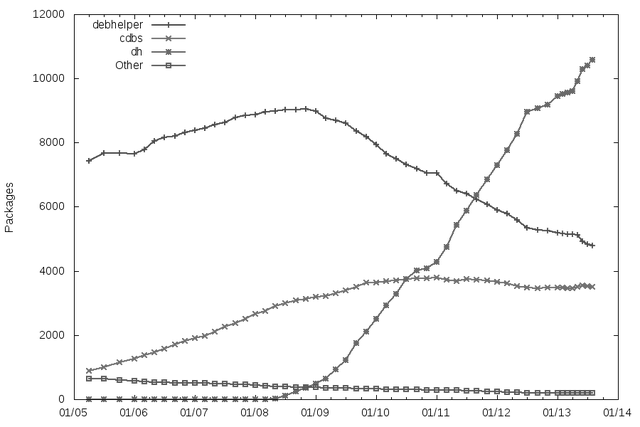
\includegraphics[width=0.5\hsize]{image201310/debian-dev-dh_mono.png}
 \end{center}
 \caption{dhによるパッケージ開発が主流}
\end{figure}
\begin{figure}[htbp]
 \begin{minipage}{0.5\hsize}
  \begin{center}
   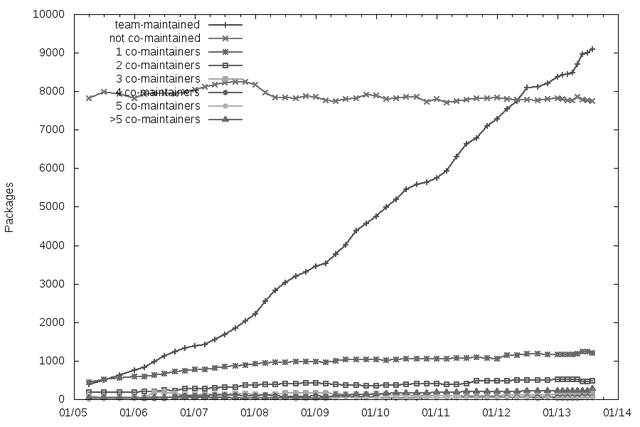
\includegraphics[width=80mm]{image201310/debian-dev-group_mono.png}
  \end{center}
  \caption{グループでパッケージ開発が主流に!}
 \end{minipage}
 \begin{minipage}{0.5\hsize}
  \begin{center}
   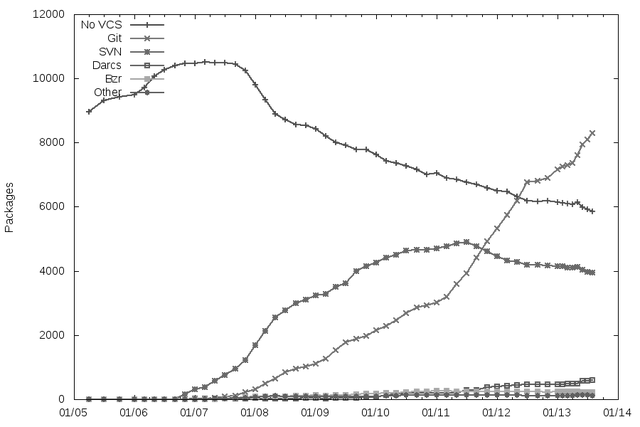
\includegraphics[width=80mm]{image201310/debian-dev-git-major_mono.png}
  \end{center}
  \caption{VCSはgitが主流}
 \end{minipage}
\end{figure}

% debian-dev-group.pngの画像は以下からダウンロード
% lucusのプレゼン資料
% http://www.lucas-nussbaum.net/blog/wp-content/uploads/2013/10/owf.pdf
% debian-dev-git-major.pngの画像は以下からダウンロード
% lucusのプレゼン資料
% http://www.lucas-nussbaum.net/blog/wp-content/uploads/2013/10/owf.pdf

% debian-dev-git-major.pngの画像は以下からダウンロード
% lucusのプレゼン資料
% http://www.lucas-nussbaum.net/blog/wp-content/uploads/2013/10/owf.pdf

\newpage

\subsection{Debian 20歳}
\begin{center}

\Large{2013年8月16日。Debian 20歳。}\\
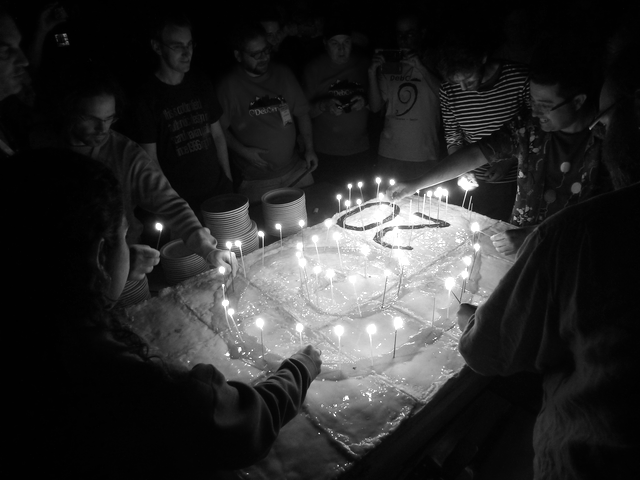
\includegraphics[width=0.8\hsize]{image201310/debian-20years_mono.png}
\end{center}
% debian-20years.pngの画像は以下からダウンロード
% lucusのプレゼン資料
% http://www.lucas-nussbaum.net/blog/wp-content/uploads/2013/10/owf.pdf

\subsection{Debian Conference 2013}

 今回はスイスで2013/8/11-8/18まで開催されました。

\begin{center}

\includegraphics[width=0.8\hsize]{image201310/DebConf13-logo_mono.png}
\end{center}

%DebConf13-logo.pngは、http://debconf13.debconf.org/artwork.xhtmlより。
%CC BY-SA 3.0とのこと。

\subsection{Debian Conference 2013の様子}

  \begin{itemize}
    \item 会場でのスケジュール詳細↓\\
       \url{http://penta.debconf.org/dc13_schedule/}
    \item ビデオもあるよ!↓\\
       \url{http://www.irill.org/videos/debconf13}
    \item 一部だけど英語の字幕もあるよ?↓\\
     \url{http://wiki.debconf.org/wiki/Videoteam/Subtitles}
  \end{itemize}

\subsection[containsverbatim]{Debian Conference 2013ビデオ視聴Tips}

 ヒアリング苦手な人は英語の字幕つかってみよう!

以下はtotemでの例:

 Step 1.  字幕の使えるプレーヤー(例:totem)とか用意する。
     \begin{commandline}
$ sudo apt-get install totem
     \end{commandline}

 Step 2.  動画をもってくる。(例:Bit from DPL)
     \begin{commandline}
$ wget http://www.irill.org/media/debconf13/Bits_from_the_DPL.webm
     \end{commandline}
 Step 3. 字幕をとってくる
     \begin{commandline}
$ sudo apt-get install git
git clone http://anonscm.debian.org/git/debconfsubs/debconfsubs.git
(あるいは、http://anonscm.debian.org/git/debconfsubs/debconfsubs.git
をブラウザで開いてsnapshotというリンクからtgzファイルを落としてくる)
     \end{commandline}

Step 4. totemにStep 2.の動画を指定して起動してstopボタンを押す。\\

Step 5. totemの「表示」$\rightarrow$ 「字幕」 $\rightarrow$ 「字幕の選択」を選択し、Step 3.で取ってきた対応する字幕ファイル(.srtファイル)を指定する。\\

Step 6. totemの再生ボタンをそのまま押すと字幕(英語)が現れる。
\begin{center}
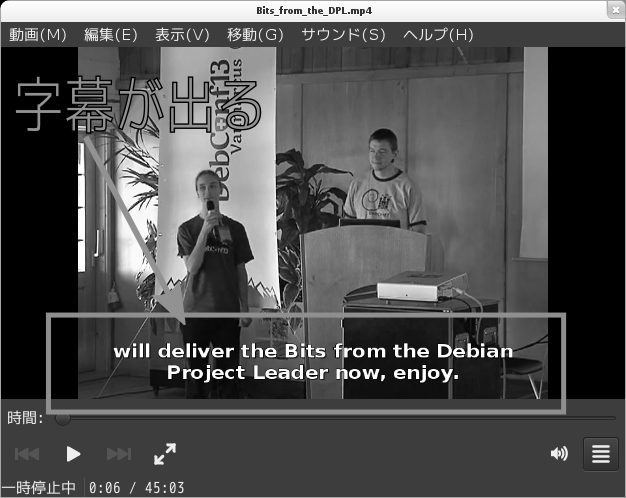
\includegraphics[width=0.5\hsize]{image201310/totem-subtitle_mono.png}
\end{center}

\subsection{Debian Conference 2013トピック紹介}
とりあえず、見どころをいくつか

\subsubsection{Bit from the Debian Project Leader}

 まずは、 ``Bit from the Debian Project Leader'' から、
(プレゼン資料:\url{http://www.lucas-nussbaum.net/blog/wp-content/uploads/2013/08/bits.pdf})
\begin{enumerate}
\item Debianの紹介と、現在のDebianのコミュニティの様子について説明(割と宣伝な感じです)
\item 現在のDebianの課題と提案
\begin{itemize}
  \item CloudのIaaS/PaaS/SaaS環境の元でどうやって自由を獲得するのか?
  \item テスト版(testing)を利用してローリングリリースとしたらどうか?(もちろん、安定版(stable)はちゃんと残す)
  \item いろいろマンパワーが足らないので、とにかく新しい開発者/貢献してくれる人を捕まえよう
 \item Debianの運営について、DPLの負荷減らしも含めて、もっとうまいこと改善したい。
\end{itemize}
\end{enumerate}

テスト版(testing)使ったローリングリリースの件は、皆さん関心が大変高いようで、
質疑応答がすべてローリングリリースの件になってました...

\subsubsection{Lightning talk}

 Debconf13のLightning talkがおもしろかったのでいくつか...

\begin{itemize}
\item Coqelicot \\
\url{https://coquelicot.potager.org}\\
※Coqelicotはフランス語でひなげしの花の意味\\
いわゆるWebベースのファイル共有サービスのプログラムを作ったとのこと。
特徴として、ファイルは全部暗号化されてストア(しかも暗号化キーはストアされない)、
時間がたてば自動で消去、消去の時にはzeroで埋めるなどの
特徴がある。ライセンスはAGPL。
\item notmuch \\
\url{http://notmuchmail.org/}
大量のメールを高速に扱うためのソフトウェアの紹介。
vim/emacsのフロントエンドなどもある。タグづけにも対応。
\end{itemize}

\begin{itemize}
\item  messaging bus system for debian infrastracture\\
\url{http://www.fedmsg.com/en/latest/}\\
Fedora PJのインフラを支えるために作られたメッセージバスシステムの紹介。
Debianにもいかが?という内容。
debianを支えるいろいろなインフラ上の仕組み(ftpキューとか、bugreportとか)
で発生する様々なイベントをこのバスシステムに流し込むと、いろいろなメディア
に柔軟に接続することができる。\\
(例:ftpキューでリジェクトされたら、WEBにも出るとかのシステムが作りやすく
 なる)\\
\url{http://www.fedmsg.com/en/latest/topology/}
を観るとわかりやすい。また、\\
繋げることができるようになったシステムの一覧↓\\
\url{http://www.fedmsg.com/en/latest/status/}
発表長すぎて司会(ドラ娘)に止められたのが残念。
\end{itemize}

\begin{itemize}
\item dedup.debian.netの紹介\\
\url{http://dedup.debian.net/}\\
バイナリパッケージ内部のファイルのmd5sumとかsha1とかのハッシュ
をとり、他のバイナリパッケージに重複したものがあるかどうかを
調べるサイトの紹介。例として、freefem++,calibreの
パッケージについて、どの程度他パッケージにも含まれている
ファイルがあるかをデモ。gzipされたファイルも元ファイルの
md5sumなどを取って比較できる。\\
例:\url{http://dedup.debian.net/binary/freefem++}\\
    \url{http://debdup.debian.net/compare/calibre/python-odf}\\
   (calibreとpython-odfは見てのとおり重複しまくり)\\
\end{itemize}

\begin{itemize}
\item Skarphed - Webmanagement system\\
\url{http://www.skarphed.org/}\\
Webサイトを非常に簡単に構築できるシステムを開発したとのことで、そのデモの紹介。
登録したサーバーに、非常に簡単にWebサイトを構築できる。AGPLで提供とのこと。
\item organaize of your life with org mode.\\
\url{http://orgmode.org/ja/}\\
emacsで動く、独特なテキスト文章作成環境のデモ。今回プレゼンすら、org modeでやった。
見ればわかりますが、TODO作成など、とても便利そうな印象を受けます。
\end{itemize}

\begin{itemize}
\item openhatch\\
\url{https://openhatch.org}\\
fossの貢献者らのためのfossプロジェクトマッチングサービスの紹介。
Web上で、fossに貢献するために必要な基本的なスキルトレーニングを
つむ、難易度に応じたfossプロジェクトを紹介する、イベントを紹介する
などのサービスが受けられる。
\end{itemize}

%$
%201310 kansai
\dancersection{git-buildpackage入門again}{佐々木 洋平}
\index{git-buildpackage}

\subsection{はじめに}

最近ではDebianパッケージの管理になんらかのバージョン管理システム(VCS)を使うことが一般的になってきました。
%
VCS usage for Debian source packages\footnote{%
  \label{footnote:1}
  (declared) VCS usage for Debian source packages:
  \texttt{http://upsilon.cc/\~{}zack/stuff/vcs-usage/}%
}によれば、
現状ではソースパッケージの $70.44\%$ がなんらかの VCS を使用しており、
そのうち $65\%$ が Git を使用しています\footnote{%
  上記URL$^{\ref{footnote:1}}$ によれば Subversion の利用が $28\%$、
  Git と subversion で全体の $93\%$ を占めています。
  近年、Subversion から Git へ移行するチームが増えていることもあり、
  dgit 含め、
  今後は Git による Debian パッケージの管理が主流となるのかもしれません。
}。
そんな訳で、Git によるパッケージ管理の知識はそろそろマストアイテムになりつつあるのかもしれません。

Debian パッケージを Git で管理するために使われるソフトウェアとして代表的なのが
\texttt{git-buildpackage} です。
これまでにも勉強会において
\texttt{git-buildpackage} に関する発表が幾つか行なわれています。
\begin{itemize}
\item 東京エリア 2007 年: 「git-buidpackage の使い方」 by 上川純一
\item 東京エリア 2008 年: 「バージョン管理ツールを使い Debian パッケージを管理する Git 編」by 岩松信洋
\item 関西 2011 年: 「vcs-buildpackage 〜Git, svn 編〜」 by 佐々木洋平
\item 関西 2011 年: 「vcs-buildpackage 〜Gitの場合(again)〜」by 佐々木洋平
\end{itemize}

当日は上記資料からの変更点ともう少し進んだ使い方について、
参加者の事前課題をベースに、
\begin{enumerate}
\item \texttt{debootstrap} を例に、 native パッケージの場合の branch について
\item \texttt{ruby-bio} を例に、Ruby 関連のパッケージでテストが転ぶ場合の対処について
\item \texttt{OpenStack} を例に、デカいパッケージの管理について
\item \texttt{yc-el} を例に、既存の vcs-buildpackage から Git への移行について
\end{enumerate}
お話ししました。

git-buildpackage は精力的に開発が進められており、便利な機能が次々と
追加されています。
興味のある方は
\begin{commandline}
  $ man gbp
\end{commandline}
% $
を読んでみて下さい。
\footnote{%
  現状は「man には書かれているけれど…」というか。
  そのうち Debian Wiki の方にも追記/更新しておきたいな、と思っています。%
}。

%201307 tokyo
%-------------------------------------------------------------------------------
\dancersection{raspbian on raspberry pi}{上川 純一}
%-------------------------------------------------------------------------------
\index{raspberry pi}
\index{armhf}
\index{raspbian}

\subsection{はじめに}

raspberry pi は市販されている安価なARMのボードです。日本国内であればRS
Components から直販されています。

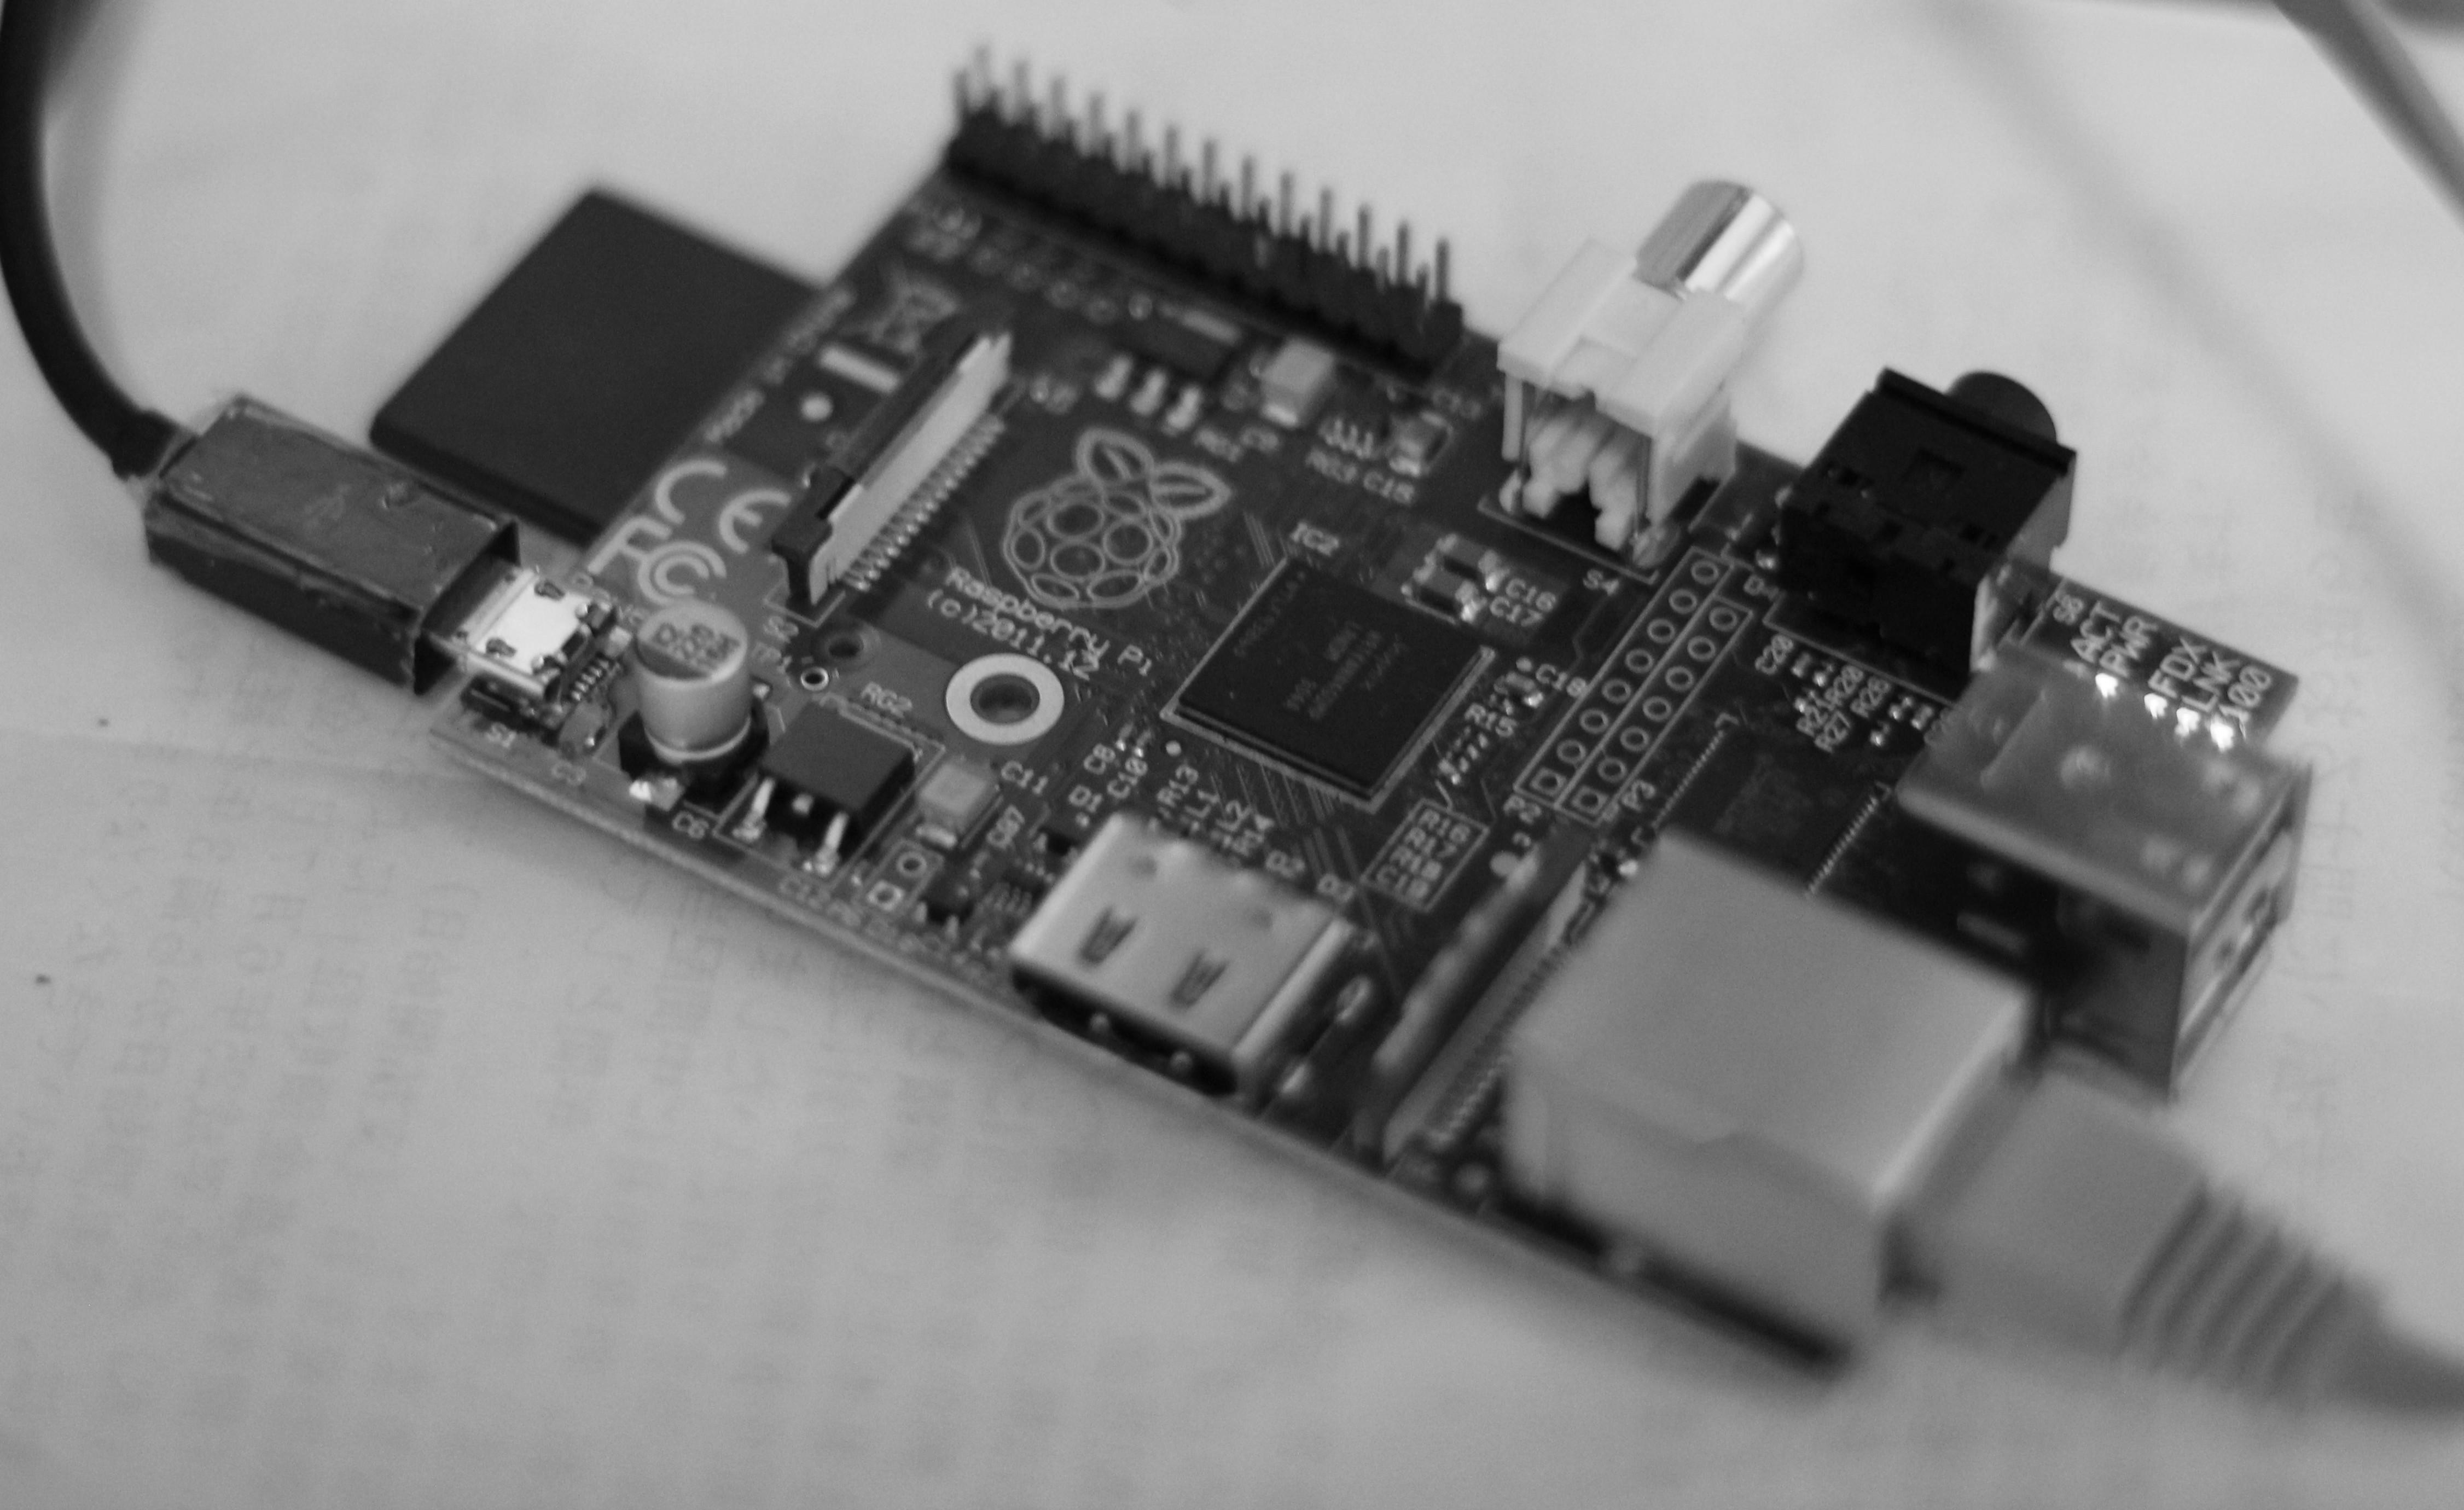
\includegraphics[width=0.5\hsize]{image201307/raspberrypi_mono.jpg}

Debianが動くデバイスという観点でみると、CPUとして ARM1176JZF-S が搭載さ
れているデバイスです。
ARM11 (ARMv6) で、ハードウェアで浮動少数点演算ができるVFPが搭載されてお
り、ARMv7 以降の機能である NEON には対応していません。

HDMI出力、イーサネット、USBホストなどがあるため、モニタとキーボードを接続
すると普通のパソコンのように利用できるようになっています。電源はmicro
USB端子で、1A以上が供給できるようになっている最近のスマートホン用の電源で
あれば流用できます。

\subsection{Raspbian}

Raspberry pi 用のLinuxディストリビューションの一つがRaspbianです。今回は
それを採用します。

\subsubsection{Raspbianでなにがうれしいのか?}

Debian そのものではなく Raspbian を利用する理由はなんでしょうか。インストール画
面がカスタマイズされていますが、それ以外に何のメリットがあるのでしょうか。
Debian GNU/Linuxのwheezy時点の安定版でサポートされているアーキテクチャは2つあり、armelとarmhfです。

raspberry pi は armel で動作します。しかし、armel は armv4 互換で、armv6 の機能を生かしてくれません。
armv6 では VFPv2 (ARMの浮動小数点ユニット) や SIMD(整数演算がストリーミング計算できる) 命令ができ
ることになっているので、それを利用しない手はないです。
一方ハードウェア浮動小数点命令を活用する設定になっているarmhfは一方でarmv7 以上でのみ動くので、armv6 では動いてくれません。

そこで登場するのがRaspbian です。これはarmv6, VFP 対応でDebianパッケージ
をコンパイルしなおしたディストリビューションです。

アーキテクチャ名はarmhf となっており、Debianのarmhfアーキテクチャのパッケー
ジをそのままインストールすることができますが、実行してもサポートされてい
ない命令を実行した時点でエラーを出力するようです。

\begin{table}[ht]
\begin{center}
\caption{各 Debian arm アーキテクチャの違い}
  \begin{tabular}{|c|c|c|c|}
 \hline
 & dpkg アーキテクチャ表示 & 浮動小数点演算ABI & 命令セットアーキテクチャ\\
 \hline
   Debian armel & armel & soft & armv4 \\
   Debian armhf & armhf & hard & armv7 \\
   raspbian & armhf & hard & armv6 \\
 \hline
 \end{tabular}
\end{center}
\end{table}

\subsubsection{インストール}

rapbian はインストール済のSDカードを入手するという事も可能ですが、そうでない場合は
本体だけでインストールが完了する手順というのはおそらくないので、別途パソ
コンを用意してください。SDカードを用意して、配布されているSDカードの起動
イメージをddで書きこみ、本体に挿入して起動するだけでよいです。
\cite{raspberrypidownloads, raspbian}

HDMIでモニターに接続して、USBでキーボードを接続して、イーサネット\footnote{
本体には物理的にRTC(時計)が搭載されていないため、起動時に現在時刻が設定
されません。ネットワークにつながっている場合はネットワークから時間を取得
することになるので通常は問題にはならないようですが、びっくりします。
}も結線
しておきます。
電源となるUSBケーブルを接続するとLEDが点灯して起動します。
しばらく起動メッセージが表示され、完了するとメニューが表示されます。

SDカードのイメージを書き込むとなるとパーティションのサイズが気になるかも
しれませんが、ファイルシステムをSDカード全体の大きさへ拡張するなどの操作
がメニューにあります。

localeの設定とかはあとで適当にやりましょう。
\begin{commandline}
$ sudo dpkg-reconfigure locales
\end{commandline}

\subsubsection{便利な小技}
\index{avahi-daemon}

raspberry pi 自体にHDMI出力やUSBなどがついているため、メイン開発機として
利用することも可能ではありますが、通常は別のマシンなどがあって作業するこ
とになると思います。
そのときに便利なのが avahi-daemon と sshfs です。

avahi-daemon をいれておけばmdns対応のクライアントからなら
``raspberrypi.local'' というホスト名で接続できるように
なります。

sshの設定はするだろうから、sshfs でファイルシステムをマウントしておけばファ
イルの共有が楽にできます。sshfsはsshの接続さえできればファイルシステムを
マウントできるので便利です。
個人的には最近はファイル共有は sshfs か git を使っています。
\begin{commandline}
$ sshfs corei7.local:path/to/work ./mnt/
\end{commandline}

\subsubsection{Raspbian での呼び出し規約}

Raspbian(armhf)ではarmelと違い、
浮動小数点関連の関数の呼び出し規約自体も変わり、使えるレジスタとして
r0-r31だけでなくd0-d31も利用できるようになります。

具体的なコンパイル例を見てみましょう。C++ のコード例があった場合にこれが
どうコンパイルされるかを見てみます。
\begin{commandline}
  double a = 1.1;
  double b = 2.3;
  cout << a*b;
\end{commandline}

armel: mfloat-abi=soft の場合のアセンブリの出力例。
doubleがrレジスタで扱われていて、ライブラリコールが行われています。

\begin{commandline}
  30:	e50b4018 	str	r4, [fp, #-24]
  34:	e24b1014 	sub	r1, fp, #20
  38:	e8910003 	ldm	r1, {r0, r1}
  3c:	e24b301c 	sub	r3, fp, #28
  40:	e893000c 	ldm	r3, {r2, r3}
  44:	ebfffffe 	bl	0 <__aeabi_dmul>
\end{commandline}

armhf: mfloat-abi=hard のアセンブリ出力例。
ABIが変わり、dレジスタで関数呼び出しの値が渡されるようになり、vmul で掛
け算が行われています。

\begin{commandline}
  30:   e50b4018        str     r4, [fp, #-24]
  34:   ed1b6b05        vldr    d6, [fp, #-20]  ; 0xffffffec
  38:   ed1b7b07        vldr    d7, [fp, #-28]  ; 0xffffffe4
  3c:   ee267b07        vmul.f64        d7, d6, d7
  40:   e59f0028        ldr     r0, [pc, #40]   ; 70 <main+0x70>
  44:   eeb00b47        vmov.f64        d0, d7
  48:   ebfffffe        bl      0 <_ZNSolsEd>
  4c:   e3a03000        mov     r3, #0
\end{commandline}

\subsubsection{hard float はどれくらい速度向上に貢献するのか?}

気になったので掛け算の速度をベンチマークしてみたのですが、サブルーチンを
呼び出すコードになっているarmelとvmul.64 を直接呼ぶようになっているarmhf
の違いがよくわからんでした。もっと劇的に違うと思ったのに。

\begin{commandline}
double mulbench(int iter, double a, double b) {
  double c;
  for (int i = 0; i < iter; ++i) {
    c = a * b;
  }
  return c;
}

int main(int argc, char** argv) {
  cout << mulbench(atoi(argv[1]), 1.2, 3.5) << endl;
  return 0;
}
\end{commandline}

\begin{table}
 \caption{1000000000 回 double の掛け算を行うループを実行するのにかかる時
 間(秒)、一回試行}
\begin{center}
 \begin{tabular}{|c|c|c|c|}
 \hline
 & armel & armhf & amd64(corei7) \\
 \hline
 -O1 & 4.5 & 4.6 &  0.35 \\
 -O0 & 134 & 130 &  2.6 \\
 \hline
 \end{tabular}
\end{center}
\end{table}

\subsection{raspberry pi にデフォルトで搭載されているセンサー}

Raspberry pi は外部センサーを付けないと何もできない感じがしますが実は一
部計測できるものもあります。
電圧とCPUの温度がそれです。

温度を表示してみましょう。ミリ度C で表示されるようです。今の温度は55度の
ようです。
\begin{commandline}
$ cat /sys/class/thermal/thermal_zone0/temp
 55148
\end{commandline}

時系列で温度のグラフを作ってみました。

\begin{figure}[H]
 \begin{center}
  \includegraphics[width=0.5\hsize]{image201307/temperature.eps}
  \caption{Raspberry pi CPU 温度(℃)の時系列での変化}
 \end{center}
\end{figure}

この温度センサーの値は0.001℃単位(m℃?)で取得できますが、結果を見た限り
では実際に取得できる値は連続ではなく離散的で、538 m℃ 単位のようです。

\subsection{おわりに}

Raspberry Piを購入してみて二ヶ月くらい放置していたのですが、いいかげんた
ちあげて見ました。しかしまだ長期的に何をさせるのかは考え中。

\begin{thebibliography}{}
 \bibitem{raspberrypidownloads} raspberry pi のソフトウェアダウンロードサイト (raspbianへのリンクが貼ってある)
\url{http://www.raspberrypi.org/downloads}

\bibitem{raspbian} raspbian のサイト \url{http://www.raspbian.org/}
\end{thebibliography}

%201307 tokyo
%-------------------------------------------------------------------------------
\dancersection{Debian linux kernel / armmp フレーバ}{岩松 信洋}
%-------------------------------------------------------------------------------
\index{armmp}

\subsection{はじめに}
Debian linux kernel の 3.9 から armhf アーキテクチャに armmp (ARM Multi Platform)
フレーバが入りました。
本稿では armmp の仕組みと対応方法について説明します。

\subsection{arm multi platformとその仕組み}

Linux kernel バージョン 3.8 ぐらいからarm multi platform(以下、ARMMP) サポートが入りました。
これは一つの linux kernel バイナリで複数のARM Soc、ターゲットボードをサポートする仕組みです。
今のところ、mvebu (Marvell SoCs)を筆頭に Versatile Express、OMAP などがサポートされて
います。バージョン3.11 ではほとんどのARM SoCがサポートされる予定になっています。

複数SoCやターゲットボードへの対応方法ですが、これはカーネル起動時にDevice Tree (以下、DT)と
呼ばれるハードウェア情報を渡すことによって、カーネルを各デバイス向けに初期化し動作するように
なります。

\subsubsection{ARMMP カーネルの起動方法}
通常Linuxカーネルを起動する場合、zImage だけで起動しますが、ARMMPや最近のARM向けカーネルはDTが
必要になっています。
DTを絡めたカーネル起動方法は3つほどあります。起動方法別にLinux上での操作(linux\$がlinux上での操作)
とU-Boot
\footnote{U-Boot は ARM 組込機器でよく利用されるブートローダ}
上での操作
(u-boot\$はU-boot上での操作)
を以下に紹介します。

\begin{enumerate}
\item zImageにdtb (DT blob。DTのバイナリ)を付加する。そしてそのzImageで起動する。\\
まずカーネルのCONFIG\_ARM\_APPENDED\_DTBが必要です。有効になっていない場合は有効にしましょう。
そしてビルドされたzImageとdtbを結合します。
\begin{commandline}
linux$ cat arch/arm/boot/zImage arch/arm/boot/dts/armada-xp-openblocks-ax3-4.dtb  > arch/arm/boot/zImage+dtb
\end{commandline}
%$
上で作成した zImage+dtb をターゲット機器上にコピーします。以下の例は tftp を使って0x2000000にコピーしています。
0x2000000 はターゲットによって異なるので環境に合わせて変更してください。
そして\texttt{go} コマンドに ロードしたアドレスを指定して実行し、カーネルを起動させています。

\begin{commandline}
u-boot$ tftpboot 2000000 zImage+dtb
u-boot$ go 2000000
\end{commandline}
%$

比較的新しいU-Boot では zImage をメモリからブートさせるためのコマンド、\texttt{bootz} があります。
カーネルイメージのチェックや初期化などを行うので bootz が提供されている場合はこちらを使う
ほうがよいです。

\begin{commandline}
u-boot$ tftpboot 2000000 zImage+dtb
u-boot$ bootz 2000000
\end{commandline}
%$

\item 1. で作成したzImage を uImage に変換して起動する。

以下は 結合したイメージを uImage 形式に変換しています。
最初の\texttt{make uImage}では zImage を uImage に変換していますが、その後zImageとdtbを結合(zImage+dtb)し、
\texttt{arch/arm/boot/.uImage.cmd}を使って結合したイメージをuImage(uImage+dtb)に変換しています。
\footnote{後述するmkimageを直接呼んでもよい}
\begin{commandline}
linux$ make uImage
linux$ cat arch/arm/boot/zImage arch/arm/boot/dts/armada-xp-openblocks-ax3-4.dtb  > arch/arm/boot/zImage+dtb
linux$ `cut -f 3- -d ' ' < arch/arm/boot/.uImage.cmd | sed -e 's/zImage/zImage+dtb/g' -e 's/uImage/uImage+dtb/g'`
\end{commandline}
%$

起動に利用するフォーマットがuImage形式の場合、\texttt{go}コマンドではなく \texttt{bootm}コマンドのを使います。

\begin{commandline}
u-boot$ tftpboot 2000000 uImage+dtb
u-boot$ bootm
\end{commandline}
%$

これらの方法は ARMMP ではない SoC単体でDTを使う場合のみ有効です。
カーネルがロードされるアドレスなどはSoCやボード毎に異なるのですが、SoC単体では
カーネルのコンフィグ情報としてこれらを持っているので上記の説明で uImage が作成できます。
しかしARMMPの場合はSoC毎にこれらの値が異なるのでターゲットSoC毎にこれらの値を変更する
必要があります。ARMMP で実行すると以下のようなエラーになるでしょう。

\begin{commandline}
linux$  `cut -f 3- -d ' ' < arch/arm/boot/.uImage.cmd | sed -e 's/zImage/zImage+dtb/g' -e 's/uImage/uImage+dtb/g'`
  CHK     include/generated/uapi/linux/version.h
  CHK     include/generated/utsrelease.h
make[1]: `include/generated/mach-types.h' is up to date.
  CALL    scripts/checksyscalls.sh
  CHK     include/generated/compile.h
  Kernel: arch/arm/boot/Image is ready
  Kernel: arch/arm/boot/zImage is ready
multiple (or no) load addresses:
This is incompatible with uImages
Specify LOADADDR on the commandline to build an uImage
make[1]: *** [arch/arm/boot/uImage] Error 1
make: *** [uImage] Error 2
\end{commandline}

ロードアドレスなどの情報はmkimage
\footnote{U-Boot 用のイメージを作成するツール。}
で指定できます。
\footnote{arch/arm/boot/.uImage.cmd 内では mkimage を呼んでいる}

\texttt{-a} でロードアドレス、\texttt{-e}でエントリポイントアドレスを指定します。
\begin{commandline}
linux$ cat zImage foo.dtb > zImage+dtb
linux$ mkimage -A arm -O linux -T kernel -C none -a 0x2000000 -e 0x2000040 -n 'Linux-marvell' -d arch/arm/boot/zImage+dtb \
arch/arm/boot/uImage+dtb
\end{commandline}
\footnote{カーネル開発者は./scripts/mkuboot.sh を使う事が多いかも。}
%$

\item uImage と dtb blob 別に読み込んで起動する。

ARMMP は 一つのバイナリで複数のARM SoC、ボードをサポートすることが目的なので、上記の方法ではサポートできません。
よって、uImage と dtb blob を分けて起動させるのが理想です。
U-Boot の場合は カーネルを起動するコマンド\texttt{bootm} を使います。

\begin{commandline}
linux$ mkimage -A arm -O linux -T kernel -C none -a 0x2000000 -e 0x2000040 -n 'Linux-marvell' \
-d arch/arm/boot/zImage arch/arm/boot/uImage
\end{commandline}
%$

\begin{commandline}
u-boot$ tftpboot 2000000 uImage
u-boot$ tftpboot 3000000 dtb
u-boot$ bootm 2000000 - 3000000
\end{commandline}
%$
%$

bootmコマンドの 第1引数はuImage がロードされているアドレス、第2引数は uInitrd(initrd イメージのuImage)がロードされている
アドレス、第3引数には dtb がロードされているアドレスを指定します。\texttt{-}は 指定なしを意味します。

ちなみにdtb の格納されてるアドレスはブートローダによってカーネル起動時の \texttt{r2} レジスタに設定され、カーネルが指定されているアドレスから
データを読み込み起動する用になっています。これは Linux カーネルの \texttt{Documentation/arm/Booting} に書かれています。

\end{enumerate}

\subsubsection{カーネルモジュールの対応}

カーネルモジュールもDTによって設定できます。
必要なカーネルドライバを組み込みにしてカーネルを起動させるのもよいのですが、ARMMPの場合
カーネルが肥大化しますので、SoCのコア部分は最低限の機能は組み込みに設定し、各デバイス用
ドライバはモジュールにしてinitrd などからロードするようにするのがよいでしょう。
Debianの場合はサポートボード毎にzImage を用意せず、上記の方法で対応しています。

\subsection{Debianでのサポート}

Debianのarmhf アーキテクチャの armmp フレーバ は上記で説明した機能を持ったカーネルをサポートするためのものです。
今回 Plat'Homeさん\footnote{\url{http://www.plathome.co.jp/}}
の Openblocks AX3 をDebianでサポートするために実装しました。
AX3 は \texttt{mvebu} という Marvell製 SoC をまとめている SoC アーキテクチャとしてサポートされているのですが、
これはARMMP サポートのみで実装されているので、Debian側でもARMMPサポートする必要がありました。
また、他の今後ARMカーネルはARMMPに移行することが決定していたので、誰かやる必要があったというのも理由の一つです。

\subsection{Debianでのカーネル提供と利用方法}
Debian はカーネルイメージを uImage で提供していません。
uImage で提供した場合、カーネルがロードされるアドレスが固定値になってしまうので、複数のデバイスをサポート
できません。Debianでは カーネルをzImage(vmlinuz) として提供しています。

しかしこのままでは U-Boot を使ったデバイスなどで使う場合に手間がかかるので、
Debian では flash-kernel\footnote{\url{http://packages.qa.debian.org/f/flash-kernel.html}}
パッケージでサポートしています。

flash-kernel は設定されたデータをもとにカーネルやinitrdをU-Bootなどで扱える形式に変換し、
フラッシュメモリに書き込む機能等を提供します。

データの形式は以下のようになります。このデータは\texttt{/usr/share/flash-kernel/db/all.db}に
記述されます。

\begin{commandline}
Machine: Marvell Armada 370/XP (Device Tree)
Kernel-Flavors: armmp
DTB-Id: armada-xp-openblocks-ax3-4.dtb
DTB-Append: yes
U-Boot-Kernel-Address: 0x2000000
U-Boot-Initrd-Address: 0x0
Boot-Device: /dev/sda1
Boot-Kernel-Path: /boot/uImage
Boot-Initrd-Path: /boot/uInitrd
Required-Packages: u-boot-tools
Bootloader-Sets-root: no
\end{commandline}

flash-kernel を実行すると設定されているデータと起動しているカーネル情報
(/proc/cpuinfo、または/proc/device-tree/model)を元にカーネルとinittd を
変換し、インストールします。
\begin{commandline}
linux$ cat /proc/cpuinfo | tail -3
Hardware        : Marvell Armada 370/XP (Device Tree)
Revision        : 0000
Serial          : 0000000000000000

linux$ flash-kernel
flash-kernel: installing version 3.10-1-armmp
Generating kernel u-boot image... done.
Installing new uImage.
Generating initramfs u-boot image... done.
Installing new uInitrd.
Installing new dtb.

linux$ ls /boot
System.map-3.10-1-armmp  initrd.img-3.10-1-armmp  uInitrd
config-3.10-1-armmp      uImage                   vmlinuz-3.10-1-armmp
\end{commandline}
%$

flash-kernel によって作成されたイメージを使った起動方法はボード毎に異なります。
OpenBlocks AX3の場合は以下の方法でSSDから起動できるはずです。

\begin{commandline}
u-boot$ ide reset
u-boot$ ext2load ide 0 2000000 /boot/uImage
u-boot$ ext2load ide 0 3000000 /boot/uInitrd
u-boot$ bootm 2000000 3000000
\end{commandline}


\subsection{終わりに}

ARMMP の仕組みと、Debianの対応方法について説明しました。\\
\sout{flash-kernel のデータはぷらっとホームさんと相談して入れようと思っているのでまだコミットされていません。\\
数日後にはパッチがBTSに上がるでしょう。OpenBlocks A6 もサポートします。\\
また、エントリーポイントを設定する項目と\\
DT の model を指定する項目がないのでこれも対応する必要があります。\\
パッチはつくってあるので後日BTSします。\\
あと、残作業としてはカーネル 3.10 では mvebu が動作しない\\
(他でも同じかも)のでパッチを当てる必要があります。\\
(コミット: \texttt{faefd550c45d8d314e8f260f21565320355c947f})。\\
これもBTSします。ということでまだまだやることはたくさんあります。}\\
既にこれらのパッチは取り込まれ、flash-kernel で ARMMP とOpenBlocks AX3がサポートされました。


%201308 kansai
\dancersection{puppet による構成管理の実践}{倉敷 悟}
\index{puppet}

\subsection{概要}

このセッションでは、まっさらな Wheezy 環境に puppet をセットアップし、
実際にマニフェストを書いて、Debian アーカイブの部分ミラーを構成させる
ところまで、実際に手を動かしながら実習していきます。

\subsection{完成図の検討}

まずは、構成管理としてやりたいことを検討します。今回のお題は、Debian
アーカイブの部分ミラーを構成する、ということになりますので、ざっくりと
下記のような構成で検討してみます。

\begin{itemize}
\item
  アーキテクチャは amd64 のみ
\item
  ディストリビューションは Wheezy (更新も含む)
\item
  とりあえず必要最低限 (required) のパッケージだけをミラーする
\item
  リポジトリの管理ツールとして reprepro を使う
\item
  puppet は reprepro の環境設定のみ行う。ミラー実行は (とりあえず) 手動
\item
  ミラーへのアクセスは http
\end{itemize}

細かいところは、多少は好みで変更してもらっても構いません。ただしミラー
対象を増やしたいのであれば、回線がリッチな時をおすすめします。

上記に付随して、

\begin{itemize}
\item
  Web サーバは apache2 を使う
\item
  Secure Apt のために GPG 設定が必要
\item
  配置場所は /var/www/debian で所有者 www-data にする
\end{itemize}

といったことも要件として検討しておく必要があります。

他にもあるかも知れませんが、おいおい加えていくこともできますので、
ひとまずこれくらいの想定で進めます。

\subsection{puppet のインストールと編集環境のセットアップ}

まずは、適当なファイルにマニフェストを書き殴りましょう。

今回、puppet はスタンドアローンでバッチ的に動作させる形で使います。
そのため、puppet のコマンドラインクライアントをインストールしてください。
また、構成管理する OS 上でマニフェストの操作も行いますので、好みの
テキストエディタをインストールします。emacs であれば、puppet-el
\footnote{vim の場合は vim-puppet} というパッケージを使うと、予約語の
色分けなどをしてくれるので便利です。
作業を記録するためにバージョン管理システムもインストールしておきましょう。

\begin{commandline}
$ sudo apt-get install puppet emacs puppet-el git tig

$ mkdir kdm201308
$ cd kdm201308
$ git init
\end{commandline}
% $

\subsection{全体像を下書きしてみる}

最初に考えたおおよその完成イメージを実現するため、トップレベルのマニフェ
ストを「こう書けたら嬉しい」という感じで下書きしてみます。

先程作成しておいたディレクトリで、site.pp というファイルを編集して
いきます。

\begin{commandline}
$ mkdir manifests
$ emacs manifests/site.pp
\end{commandline}

\begin{commandline}
# 必要になりそうなパッケージを class として列挙
class {
  'apache2':;
  'reprepro':;
  'gnupg':;
}

# reprepro のミラーディレクトリをよしなに設定 (してほしい)
reprepro::mirror { '/var/www/debian':
  owner => 'www-data', group => 'www-data',
  architecture => 'amd64',
  distribution => 'wheezy',
  partial => 'required',
}

# apache のミラー公開用サイトを追加 (してほしい)
apache2::site {
  'mirror':
    content => '後で';
}
\end{commandline}

要するに、やりたいことは、

\begin{itemize}
\item reprepro でいい感じのミラーを作る
\item 作ったディレクトリを適当に Web アクセスできるようにする
\end{itemize}

ということですね。

とりあえず並べた class の要素はまだ存在しないため、このままでは
実行できません。それぞれ作ってあげる必要があります。

ひとまず、作業を git に入れておきましょう。ログは好きなように書いて
ください。

\begin{commandline}
$ git add site.pp
$ git commit
\end{commandline}

このあたりで、必要そうであれば、前回のおさらいも兼ねて puppet のマニフェスト
書式について口頭で簡単なおさらいをします。資料としては前回の分 (2010/06) を
参照してください。

\subsection{必要な class を作る}

さて、ここからが本番です。何はともあれ、不足している class 定義の枠と、
インストールするパッケージの指定だけしてみましょう。

\begin{commandline}
class apache2 {
  package { 'apache2':; }
}

class reprepro {
  package { 'reprepro':; }
}

class gnupg {
  package { 'gnupg':; }
}
\end{commandline}

これだけでも、とりあえず必要なパッケージは入ります。凝ってみたいなら、
リファレンスを見ながらパラメータを追加してみてもいいでしょう。

これだけでは、パッケージ固有の設定は debconf 任せになってしまいますので、
設定を追加するために、都合のよいリソース定義が必要になります。
まずは、全体像で書いたリソースを受ける枠をとりあえず作って……

\begin{commandline}
define reprepro::mirror (
  $owner,
  $group,
  $architecture,
  $distribution,
  $partial
  ) {

}

define apache2::site (
  $content
  ) {

}
\end{commandline}

それぞれの内部をどのように構成するか考えてみましょう。この
セッションでは、かなりやっつけ感の高い構成で流してしまいますが、
実際にマニフェストを書くときは、構成管理しようとしている対象の
パッケージの動きをしっかり観察するようにしてください。

ここにファイルを置くためには、このパッケージが入っていなくては
ならない、このファイルはこういうパーミッションで置かれている、
このリソースの後にこういう処理が必要だ、パッケージの削除が失敗
しないか、などなど……。\footnote{パッケージシステムとの整合を
とる話は、それだけでセッションが成立する程度にはトピックがある
ので、また別の機会に。}

構成管理をしっかり書こうと思えば、その対象をよく知っておく必要
があります。そこの手間が省けるツールではないので誤解のないように
しましょう。
ありもののレシピ使い回せばいいんじゃんウェーイ、という考え方も
ご時世としてはありなのかも知れませんが、その後の運用を誰かに
押しつけてトンズラできる環境でないのならばオススメしません。

さて、構成管理ツールが流行するよりも前から、dpkg はその一部を
担っているという経緯もありますので、

\begin{itemize}
\item 一部、やってることが puppet と被る(プロセスの起動制御など)
\item 設定方針が debian policy で決まっているため、やりたい設定と矛盾す
る場合がある
\end{itemize}

といったあたりに注意して、設定を煮詰めていきましょう。

\subsubsection{apache2}

実は、今回はいろいろな前提の上にのっかっているため、apache2 に
追加の設定は不要です。デフォルトのままで、reprepro によって作成
されるミラーにそのままアクセスできるはずです。

ただ、それだとさすがに味気ないですから、簡単にサイト設定の仕組みを
追加してみましょう。これは Debian においては、
/etc/apache2/sites-\{enabled$|$available\}/ ディレクトリと
a2ensite/a2dissite コマンドによって制御されている部分ですね。

きっちり書くなら、available ディレクトリに file リソースの content で
ファイルを配置し、ensure パラメータの内容によって enable/disable を制御
する exec リソースを書いておく、といったことをすればいいと思います。
ただし、今回は面倒なので単純に「content の内容を直接 sites-enabled に
つっこむ」だけにしておきます。

すると、おおよそ次のようになるかと思います。

\begin{commandline}
define apache2::site (
  $content
  ) {

  file { "/etc/apache2/sites-enabled/${name}":
    content => $content,
    require => Package['apache2'],
    notify  => Service['apache2'],
  }
}
\end{commandline}

設定ファイルを変更したら、プロセスも再起動して欲しいので、notify
も追加しました。この Service はまだ定義していないので、class の方に
対応する定義を書いておきましょう。

\begin{commandline}
class apache2 {
  package { 'apache2':; }
  service { 'apache2':; }
}
\end{commandline}

これで、apache2 の
\begin{itemize}
\item パッケージを入れ
\item 適当なサイト設定を行い
\item サービスを起動する
\end{itemize}
簡単な class が出来ました。

後は、実際に流しこむサイト設定を用意する必要があります。今回は、さきほど
書いたようにデフォルトのままでも動くので、そのままデフォルト設定をパクっ
ておくことにします。

一度 apache2 パッケージをインストールし、sites-available/default
ファイルをコピーしましょう。

\begin{commandline}
$ sudo apt-get install apache2
$ cp /etc/apache2/sites-available/default site-mirror.erb
$ sudo apt-get purge apache2 && sudo apt-get autoremove
\end{commandline}

このファイルをテンプレートとして content に渡してあげたいので、
所定の場所に配置した上で、マニフェストから読みこむようにして
おきます。
\begin{commandline}
$ mkdir templates
$ mv site-mirror.erb  templates

apache2::site {
  'mirror':
    content => template('site-mirror.erb');
}
\end{commandline}

これで、apache2 については一応完成です。このあたりで、git commit して
おきましょう。

パラメータの渡し方、ファイルの指定方法などは、選択肢がいくらでも
あって、正解はありません。かけられる時間や、どれくらい類似度の高い
構成を繰り返すのか、などマニフェストを作成する状況にあわせて調整
するようにしてください。\footnote{実例としてあげている処理は、考慮
の足りない、ダメなやっつけ仕事の例ですので、反面教師として頂ければ……}

\subsubsection{reprepro}

今回は reprepro 自体の使い方は主眼ではないので、簡単に紹介だけしておきます。

reprepro は、指定したディレクトリに Debian のミラーを構成するツールです。
指定ディレクトリに決まったフォーマットで設定ファイルを用意しておけば、
柔軟にミラーを構成できます。そのため、ちょっと手元でとか社内利用などの
用途で、気軽にミラーを用意することができます
\footnote{パブリックなフルミラーを用意したい場合は、別途専用のツールがあります}。

イメージできるほど対象のソフトウェアに馴染んでいない場合は、まず puppet
抜きで動作させてみて、挙動を把握するようにしましょう。ともあれ、手動で
reprepro をインストールします。

\begin{commandline}
$ sudo apt-get install reprepro
\end{commandline}

reprepro を動作させるために、conf/distributions と conf/updates、2 つの
設定ファイルが必要になります。
ミラーのファイル置き場にするディレクトリに移動してください。ここでは、
wheezy の部分ミラーを作成しますので、ひとまず下記の内容でファイルを
作成しましょう。

distributions には、公開する対象 (sources.list でディストリビューション
コードネームとして参照されるもの) を指定します。今回の例では wheezy と
なります。

\begin{commandline}
Codename: wheezy
Architectures: amd64
Description: wheezy-mirror
Components: main contrib
Update: wheezy wheezy-updates wheezy-security
\end{commandline}

updates には、ミラーに含めるパッケージを取得してくる上流のリポジトリを
指定します。

\begin{commandline}
Name: wheezy
Method: http://ftp.jp.debian.org/debian
Suite: wheezy
Components: main contrib
Architectures: amd64
VerifyRelease: AED4B06F473041FA
FilterFormula: Priority (==required)

Name: wheezy-updates
Method: http://ftp.jp.debian.org/debian
Suite: wheezy-updates
Components: main contrib
Architectures: amd64
VerifyRelease: AED4B06F473041FA
FilterFormula: Priority (==required)

Name: wheezy-security
Method: http://security.debian.org/debian-security
Suite: wheezy/updates
VerifyRelease: AED4B06F473041FA
FilterFormula: Priority (==required)
\end{commandline}

Secure APT 用の公開鍵は、次のようにしてインポートしておきます。

\begin{commandline}
$ gpg --recv-key AED4B06F473041FA
\end{commandline}

これによって、このミラーが上流からダウンロードする時に、公開鍵に
よる確認が行なわれます。

設定が終わったら、正しく動作するか確認します。

\begin{commandline}
$ reprepro -V update wheezy
\end{commandline}

少し時間がかかりますが、指定したミラーからファイルをダウンロードする
はずです。
終わったら、ノードの /etc/apt/souces.list を少しいじって、apt-get から
アクセスできるかどうか確認しておくといいでしょう。

さて、ここまでで reprepro が動作する設定ができあがりましたので、これを
puppet のマニフェストに移していきましょう。

一旦、reprepro で作成したファイル類を全て削除します(別にしなくても構い
ませんが、ここまでのテスト内容を掃除するためです)。

\begin{commandline}
$ sudo rm -r /var/www/debian
\end{commandline}

先程作成した site.pp を開き、設定ファイルを流しこむ方法を考えます。
パラメータをテンプレートで受けるなど、やり方はいくつかありますが、ここでは
単純に、ファイルをそのまま置くだけとしておきます。

ミラーは、配置するディレクトリを変更すれば、ノード内に複数作成することが
できる (べきな) ので、クラスではなく、リソースとして定義します。

\begin{commandline}
class reprepro {
  package { 'reprepro':; }
}

define reprepro::mirror (
  $distributions,
  $updates,
  ) {
  # ミラーの配置ディレクトリを作成する
  ## リソース名としてフルパスが渡されてくる想定
  file { "$name":
    ensure => directory,
  }
  -> file { "${name}/conf":
    ensure => directory,
  }
  -> file { # 設定ファイルの名前はパラメータとして受け取る
    "${name}/conf/distributions":
      content => $distributions;
    "${name}/conf/updates":
      content => $updates;
  }
}
\end{commandline}


パラメータ指定をやめてファイルを直接与えることにしたので、呼び出し元も
変更する必要があります。

\begin{commandline}
# reprepro をよしなに設定してほしい
reprepro::mirror { '/var/www/mirror':
  owner => 'www-data', group => 'www-data',
  distributions => '上で作成したファイルの内容をペースト
最後に改行が必要なので注意
',
  updates       => 'こちらも同様に
'
}
\end{commandline}

ここまでで、puppet を実行することで、reprepro の設定ファイルが準備され、
後はコマンドを実行するだけ、という状態になります。忘れないように、git commit
しておきましょう。

最終的には reprepro コマンドの実行も puppet にやらせるといいのですが、
話が広がってしまうので、今回はここまでとしておきます。

\subsection{マニフェストの適用とデバッグ}

さて、ここまでで作成したマニフェストを実行すると、

\begin{itemize}
\item apache2 がセットアップされて、ミラーのディレクトリが公開される
\item ミラーのディレクトリに reprepro の設定が用意される
\end{itemize}

はずですので、早速試してみましょう。まずは、dry run から。

\begin{commandline}
$ puppet apply -v /etc/puppet/manifests/site.pp --noop
\end{commandline}

スペルミスや、記号抜けなど、書式違いがあれば puppet が教えてくれますので、
出力内容を確認してみてください。

問題なさそうなら、$--$noop を削って、そのまま実行しましょう。

\subsection{マニフェストの整理}

puppet は、モジュールという単位でマニフェストを分割することができます。

今回は、さほど大きなマニフェストを書いているわけではないので、site.pp
だけでも十分見通しがききますが、1ファイルにダラダラ書いていくにも限度が
あります。ある程度大きく育ってきたら、マニフェストを分割しましょう。

もし実例が見たい、ということであれば、後半部分でやりますのでリクエストを
ください。

\subsubsection{パッケージモジュール}

モジュールをどういう単位で切り出すかは、個人の好みもあると思いますが、
ここではとっかかりとして「パッケージ単位」をおすすめしておきます。

では、パッケージに対応した puppet モジュールの置き場所を決めましょう。
例えば、

\begin{commandline}
$ sudo  mkdir -p /etc/puppet/modules/
\end{commandline}

などとします。このディレクトリ以下に、モジュール名のディレクトリを作成
していくことになりますが、Debian での利用を考えると、「ソースパッケージ名」
を使うといいでしょう (バイナリパッケージが細かく分割されていたりするので)。

例えば、apache2 のモジュールを作るのであれば、

\begin{commandline}
$ mkdir -p /etc/puppet/modules/apache2/manifests
$ emacs /etc/puppet/modules/apache2/manifests/init.pp
\end{commandline}

のようにします。「モジュール名/manifests/init.pp」はルールなので、別の
ファイル名にすることはできません。
とりあえず、先程作成した、apache2 クラスの内容をこちらに移動させてみて
ください。

パッケージモジュールの内容を決める上では、次のことに注意するといいでしょう。
\begin{itemize}
\item
  パッケージ固有の内容に絞り、サイト固有の設定は可能な限り含めない
\item
  後で再利用できるようにパラメータを決める
\end{itemize}

\subsubsection{サービスモジュール}

パッケージモジュールを切り離した後は、ノード/サイト固有の設定が
site.pp に残っている状態になっているはずです。そのうち、今作業している
ノードだけでなく別のノードでも再利用しそうなロール (うちでは Web サーバは
いつもこの設定で作るようにしてるんだ、とか) も、可能であればモジュールと
して切り出しておきましょう。

puppet から見ると、用途に関係なくモジュールはモジュールなのですが、
パッケージモジュールと区別するために、便宜的にサービスモジュールと呼んで
おきます。
puppet の書式ガイドライン的には、モジュール名として頭に s\_ をつける
ことになっています。

サービスモジュールはサイト固有の内容になりますので、パッケージモジュール
ほど境界を気にしなくてもいいでしょう。

例えば、部分ミラーのロールを作るのであれば、

\begin{commandline}
mkdir -p /etc/puppet/services/s_mirror/manifests
emacs /etc/puppet/services/s_mirror/manifests/init.pp
\end{commandline}

として、今回作成した reprepro の設定内容自体や、apache2 のサイト設定
などを放りこむところからはじめるといいと思います。

\subsection{ここからの育て方}

ひとまず、今回のセッションで Debian アーカイブのローカルミラーが
お手軽に作れるようになっているハズでので、次のステップとして、

\begin{itemize}
\item reprepro の設定ファイル指定がダサすぎるのでなんとかする
\item ローカルミラーを参照するように sources.list を設定する
\item ローカルミラーに独自パッケージを追加できるように reprepro の設定を追加する
\item 手動のままだった reprepro のコマンド実行をリソースに含める
\item reprepro のコマンド実行を cron に登録してみる
\item germinate を使って必要なパッケージを指定してミラーの対象にする
\end{itemize}

といった拡張からはじめていくと、とっかかりやすいのではないかと
思います。公式のリファレンスを眺めながら頑張ってみましょう。

%201311 tokyo
%-------------------------------------------------------------------------------
\dancersection{tramp入門}{上川純一}
%-------------------------------------------------------------------------------
\index{tramp}
\index{emacs}

\subsection{emacsでリモートファイル編集するTrampのすすめ}

リモートサーバでファイルの編集はどうしていますか?moshを使っている?
sshfsを使っている?いろいろあると思いますがmoshを使うとローカルのファイル
と扱いが変わってしまい、リモートのviだったりemacsを使って編集することにな
り、設定の同期がほぼ不可能になります。一方sshfsだとローカルファイルのよう
に扱うことができるのですが、rootなどの別のユーザ(root?)としてファイルの
編集ができにくかったりしますし、リモートホストでコマンドを実行しようとす
ると別途sshでログインして作業することになり、sshセッションをひらきながら
sshfsで実行し、ローカルのパスとリモートのパスの違いを意識しながら作業す
ることになります。

emacs ユーザの方々に朗報です。tramp とは \texttt{/sshx:hostname:path/to/file} とい
う特殊なファイル名を指定すると透過的にsshを使ってリモートのファイルを取
得して編集できるようにしてくれる仕組みです。
また、dired でリモートのディレクトリのファイル管理もローカルと変わらない
ように行えます。
さらに便利なのは \texttt{M-x shell}, \texttt{M-x compile} などリモートでコマンドを実行する
コマンドを利用するとhostname にsshでログインして path/to/file をカレント
ディレクトリとした状態でコマンドを実行してくれるところです。
個人的にはmoshなどを利用してシェルのコマンドを実行するより、emacsのロー
カルバッファでコマンドラインを編集して確定時にリモートに送信するスタイル
が気に入っています。

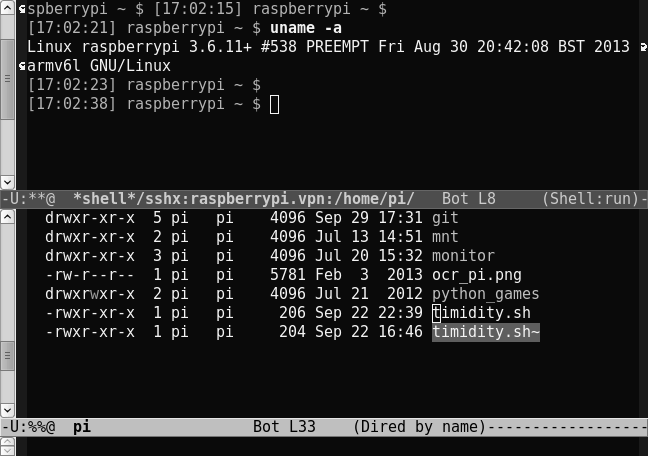
\includegraphics[width=12cm]{image201311/tramp-screenshot_mono.png}


\subsection{リモートホスト側の設定}
ssh で接続される側のの設定ですが、trampはシェルのセッションの入出力を利用し、機械的に
プロンプトを検出するので、プロンプト(PS1など)をカスタマイズしていると
動かない場合があります。trampのために \texttt{.bashrc}はシンプルにするといいかも
しれません。

例えば、raspbian のデフォルトは色がつきまくってたりしてファンシー過ぎてう
まく動きませんでした。

\subsection{sshの設定とチューニング}
\index{ssh}
\index{ssh\_config}

ローカルのsshの設定ファイル \verb!~/.ssh/config! に設定したほうがよいも
のを紹介します。
マニュアルは \verb!man ssh_config!\cite{sshconfig}で参照できます。

\subsubsection{ControlMasterで接続を再利用}

手元ではこんな設定にしています。

\begin{commandline}
 ControlMaster auto
 ControlPersist 120
 ControlPath ~/tmp/ssh-%r@%h:%p
\end{commandline}


ControlPersist に指定した秒数間、sshで接続する際にデーモンプロセスが起動
して、コネクションを張りっぱなしにし、コネクションを再利用してくれます。

手元では、ControlPathを明示的に指定しています。ホームディレクトリ以下の
tmp 以下にしているのはファイル名が予想可能になるので衝突を防ぐためです。

ControlMasterをAutoにしておくとすでにコネクションが開いていない場合はデー
モンをたちあげて、もしコネクションが開いている場合にはそれを利用するよう
になります。

リモートでtrueコマンドを実行する速度を計測してみたところ
随分高速になり(\fgref{fig:pingwagner})、ping time の二倍くらいになってくれ
るようです。

\begin{table}[ht]
\begin{center}
  \begin{tabular}{|c|c|}
   command & time(ms) \\
   ping& 271 \\
   ssh connection sharing on & 544 \\
   ssh connection sharing off & 4070 \\
 \end{tabular}
 \caption{ping test against wagner.debian.org}
 \label{fig:pingwagner}
\end{center}
\end{table}

\subsubsection{keep-alive}

trampはネットワーク接続の切断をsshプロセスの生死で検出します。
sshはネットワーク接続がきれたりしてもすぐにはそれを検出しないので、キー
プアライブを送信するようにします。

\begin{commandline}
 ServerAliveInterval 3
 ServerAliveCountMax 5
\end{commandline}


本当はパソコンがサスペンドから復活して新しいネットワーク接続につながった
らsshプロセスに再接続してほしいのですが、その方法をまだ発見できていませ
ん。

\subsubsection{その他の設定}

Mac のRendezvousとかLinuxのAvahiとか設定しているとホスト名.local という名
前で名前解決ができるようになりますが、そうするとIPアドレスはDHCPだと一定
ではないため、IPに対しての鍵が違うと怒られます。その場合はホストIPをチェッ
クしないようにするとよいでしょう。

\begin{commandline}
 Host *.local
  CheckHostIP no
\end{commandline}

あとデフォルトではいろいろな鍵を試したりする設定になっていますが、ついで
に鍵を指定して公開鍵認証にしておくとよいんじゃないでしょうか。

\begin{commandline}
 Host raspberrypi.vpn
  Hostname そのホストのIPアドレス
  IdentityFile ~/.ssh/ssh-keygenで作ったファイルのパス
  IdentitiesOnly yes
\end{commandline}


\subsection{trampの.emacs での設定とチューニング}

\texttt{.emacs} にほとんど設定しなくてもデフォルトの設定でそれなりにうご
きます。
マニュアルは info 形式で提供されています\cite{trampinfomanual}。

trampでは\texttt{/sudo:root@hostname:/} のような形式でリモートホスト上で
sudoで別ユーザになってからファイルにアクセスするように指定することが可能
です。ただ、そのためにはリモートホストへの到達手段を指定する必要がありま
す。たとえば、ローカルネットワークにあるホスト \texttt{*.local} でsudoを
サポートしたいという要望であれば、次のような設定を追記しておきます。

\begin{commandline}
 (add-to-list 'tramp-default-proxies-alist
      '("\\.local\\'" "\\`root\\'" "/ssh:%h:"))
\end{commandline}

あと、デフォルトの設定だとリモートアクセスしているというメッセージがステー
タスに表示されるのですが、正直邪魔なのでそれを消すのもよいかと思います。

\begin{commandline}
(custom-set-variables '(tramp-verbose 1))
\end{commandline}

\begin{thebibliography}{0}
 \bibitem{trampinfomanual} ``TRAMP User Manual'', info
	 page,
	 \url{http://www.gnu.org/software/emacs/manual/html_node/tramp/index.html#Top}
 \bibitem{sshconfig} ``ssh\_{}config(5)'' manual page,
\end{thebibliography}

%201309 kansai
\dancersection{Linuxとサウンドシステム}{坂本 貴史}

\subsection{ALSAの概要}
\begin{itemize}
\item Advanced Linux Sound Architecture
\item ALSAはLinuxのためのサウンドデバイスを開発するプロジェクト
\item 1998年あたりに始まる
\item LinuxディストリビューションおよびAndroidがALSAを利用してデバイスとの入出力を行う
\item 主要な開発者はLinuxディストリビューター、半導体メーカー、Androidメーカーに在籍
\end{itemize}
\index{alsa}

\subsection{音声入出力に関係するハードウェアとその制御及びデータ}
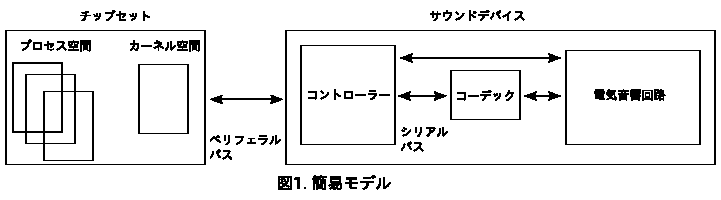
\includegraphics[width=\hsize]{image201309/alsa_mono.png}

\subsection{ALSAのユーザー/カーネル空間のインターフェイス}
\begin{itemize}
\item ALSAはLinux専用のサブシステム。Unixライクにデバイスノードへのファイル操作を行ってデバイスを操作する
\item サウンドデバイスはキャラクター型のデバイス。\texttt{/dev/snd}以下に設けられる。
\item open(2)/read(2)/write(2)/close(2)だけでデバイスを制御するのは難しい。
\item ioctl(2)で柔軟な操作を行う。libasound2で専用APIを提供。
\item procfsの\texttt{/proc/asound}以下のノードでALSAの基本情報を提供している
\end{itemize}

\subsection{Linuxカーネル/ドライバーとALSA}
\subsubsection{デバイスクラスとALSA}
\begin{itemize}
\item Linuxにはデバイスクラスがある。soundcoreモジュールがsoundクラスを提供する。ALSAはsoundクラスのドライバー。
\item ALSA Coreは各ドライバーに対し、以下の機能を提供
  \begin{itemize}
  \item ユーザー空間とのインターフェイスを提供するAPI
  \item Linuxのdriver/base(sysfs含む)に対する共通API
  \item Linuxのprocfsに対する共通API
  \item Open Sound Systemとの互換レイヤ
  \item その他ヘルパー関数
  \end{itemize}
\item ALSAのドライバーは、Linuxの各バスドライバーが提供するAPIを利用し、ALSAのインターフェイスとデバイスを中継する役割を果たす
\end{itemize}

\subsection{ALSAのカーネルランドコンフィグレーション}
\begin{itemize}
\item ALSAのカーネルランドはLinuxのローダブルモジュールとして実装されている
\item modprobeを使い、ローダブルモジュールにオプションを渡すことができる
\end{itemize}

\subsection{ALSAのユーザーランドコンフィグレーション}

\begin{itemize}
\item libasound2は設定ファイルのパース機能を持つ
\item libasound2はシステムレベル、ユーザーレベルでランタイム設定を変更できる
\item libasound2はプラグイン構造を持つ
\end{itemize}

\subsection{ALSAのアプリケーション}
\begin{itemize}
\item alsa-utils、PulseAudio、Jack Audio Connection Kit
\end{itemize}

\subsection{圧縮データとgstreamer/libav}
\begin{itemize}
\item サウンドシステムは基本、PCMデータを扱うよう作られている
\item 圧縮データからPCM標本を取り出す処理をどこかで入れる必要がある
\end{itemize}

\subsection{Androidとtinyalsa、AudioFlinger}
\begin{itemize}
\item AndroidはカーネルランドにLinuxカーネルを使っていて、ALSAを利用している
\item ユーザーランドはlibasound2ではないtinyalsaを使う
\end{itemize}

\subsection{その他の話題}
\begin{itemize}
\item salsa、COMPRESS/tinycompress、Audio Visual Bridge (AVB)、FirewireとALSA
\end{itemize}

%201310 kansai
\dancersection{ALSAのユーザーランド解説}{坂本 貴史}

\index{libasound2}

\begin{itemize}
\item ライブラリ、設定ファイル、プラグインなどがある
\item ドキュメントはパッケージ「{\tt libasound2-doc}」で「{\tt /usr/share/doc/libaound2-doc/html/}」以下へインストールできる
\item Androidは独自にユーザーランドの実装を持っている
\end{itemize}

\subsection{ライブラリ}
\begin{itemize}
\item  asound
\item 設定ファイルのパース機能を持つ
  \begin{itemize}
  \item  システムレベル、ユーザーレベルでランタイム設定
  \end{itemize}
\item プラグインを持つ
  \begin{itemize}
  \item 任意の機能を付与できる
  \end{itemize}
\end{itemize}

\subsection{PCMノード}
\begin{itemize}
\item ランタイムに設けられる。
\item {\tt aplay -L}あるいは{\tt arecord -L}で一覧を取得できる。
\item PCMのキャラクターデバイスを隠蔽し特定の機能を付与したもの
\item この特定の機能を付与するために用いられるのがPCMプラグイン
\item 設定ファイルがPCMノードを設けている
\item ライブラリのPCMインターフェイスでハンドルを開く時に指定する
\end{itemize}
\index{arecord}
\index{aplay}

\begin{commandline}
$ aplay -L
default
    Playback/recording through the PulseAudio sound server
sysdefault:CARD=Intel
    HDA Intel, ALC889 Analog
    Default Audio Device
front:CARD=Intel,DEV=0
    HDA Intel, ALC889 Analog
    Front speakers
surround40:CARD=Intel,DEV=0
    HDA Intel, ALC889 Analog
    4.0 Surround output to Front and Rear speakers
surround41:CARD=Intel,DEV=0
    HDA Intel, ALC889 Analog
    4.1 Surround output to Front, Rear and Subwoofer speakers
\end{commandline}
\begin{commandline}
surround50:CARD=Intel,DEV=0
    HDA Intel, ALC889 Analog
    5.0 Surround output to Front, Center and Rear speakers
surround51:CARD=Intel,DEV=0
    HDA Intel, ALC889 Analog
    5.1 Surround output to Front, Center, Rear and Subwoofer speakers
surround71:CARD=Intel,DEV=0
    HDA Intel, ALC889 Analog
    7.1 Surround output to Front, Center, Side, Rear and Woofer speakers
\end{commandline}

\subsection{設定ファイル}
\begin{itemize}
\item ALSA特有の記法で書かれている
\item システムレベルは{\tt /usr/share/alsa}以下にある
  \begin{itemize}
  \item {\tt /usr/share/alsa/alsa.conf}の「{\tt defaults.namehint.extended off}」が、{\tt hw/plughw/dmix/dsnoop}の表示を抑制
  \end{itemize}
\item ユーザーレベルは「{\tt .asoundrc}」をホームディレクトリに配置
\end{itemize}

\subsection{プラグイン}
\begin{itemize}
\item プラグインには2つのタイプがある
  \begin{itemize}
  \item[PCMタイプ] PCMノードに機能を追加する
  \item[MIXERタイプ] Controlノードに機能を追加する
  \end{itemize}
\item {\tt aplay -L}でいろんなノードが見えるのはPCMプラグインのおかげ。
  \begin{itemize}
  \item[front] フロント出力のためのもの
  \item[surroundXXX] サラウンド出力のためのもの
  \item[hw] 標本化周波数、量子化ビット数、チャンネル数などをちゃんと指定する必要がある
  \item[plughw] 上記をよしなに設定してくれる
  \item[pulse] 出力をPulseAudioに流しこんだり、入力をPulseAudioから受けたりする
  \item[dmix] 複数の出力をひとつのストリームに合成する
  \item[dsnoop] ひとつの入力を複数のストリームにする
  \item[default] ALSAの配布するパッケージでは、dmix/dsnoopを入出力スレーブとしている
  \end{itemize}
\item その他のプラグイン
  \begin{itemize}
  \item[bluetooth] Bluezを利用して音声機能を持つBluetoothデバイスを使う
  \item[ladspa] LADSPAというフレームワークのプラグインを使う
  \end{itemize}
\end{itemize}

\subsection{PulseAudio}
\begin{itemize}
\item 複数のアプリケーションの出力を束ねたり、入力を分割したりする
\item 最近のデスクトップ環境は、libasound2のpulseプラグインを有効にし、defaultノードをpulseノードに設定

  こうすることで、ALSAを直接利用するアプリケーションの入出力をPulseAudioに向けている
\item PulseAudioのモジュール構造
  \begin{itemize}
  \item いろんな機能を共有ライブラリの形で提供。自在にロード・アンロードできる。
  \item \url{http://www.freedesktop.org/wiki/Software/PulseAudio/Documentation/User/Modules/}
  \end{itemize}
\item ALSA以外のサブシステムを使える
  \begin{itemize}
  \item Bluez
  \item Network
  \end{itemize}
\end{itemize}

%201308 tokyo
%-------------------------------------------------------------------------------
\dancersection{OpenVPNを使ってみた}{上川純一}
%-------------------------------------------------------------------------------
\index{openvpn}

\subsection{はじめに}

VPN(仮想プライベートネットワーク)とはインターネット上にある(WAN)に閉域ネットワー
ク(LAN)を仮想的に構築する方法です。

OpenVPNは認証と接続方式の部分でTLS\cite{rfc5246} \footnote{規格がTLSにな
るまえはSSLという規格でした}を活用しています。TLSはHTTPSなど
で利用されている仕組みで、公開鍵認証をつかって最初の鍵交換をおこな
い、そこで交換した対象鍵をつかって実際の通信をすることで効率良く暗号通信ができる
ようになっています。

\subsection{今回実現したいこと}

今回想定する例としてとある個人の開発環境ネットワーク構成図を見てみましょ
う(\fgref{fig:network})。

自宅にはごく一般的なプロバイダ契約でネットワークをひいていて、ラッ
プトップと携帯電話はどういうネットワークを経由してどういうIPアドレスでつ
ながるのかよくわからないという構成です。

携帯電話とラップトップから自宅にあるサーバ Raspberry Pi にアクセスできる
ようにしたい、そう思った時にプライベートIPで接続しているプロバイダー接続がネッ
クになります。

開発や実験などに便利な環境を実現したい、それはRaspberry pi とラップトップ
と携帯電話が同じLANにいるような環境です。

\begin{figure}[H]
\begin{center}
  \includegraphics[width=0.8\hsize]{image201308/network.eps}
 \caption{とある個人の開発環境ネットワーク構成図}
 \label{fig:network}
\end{center}
\end{figure}

\subsection{OpenSSL, CA の仕組み}

OpenVPN で利用できる認証のしくみは複数あり、一番簡単な方法は共有鍵方式だ
と思われます\footnote{認証なし暗号化なしという方法もあってそっちのほうが
簡単ですがopenvpnの接続性テスト以外ではあまりつかわないと思います}。ここ
では自分の直接の管理下にあるマシンを複数台管理する場合に便利そうな方式、
自前でCAを立ててPKI(x509)で構築する方法について紹介します。

今回紹介する方式を実現する副作用として、openvpnに脆弱性があったり、認証情
報がもれると外部のユーザが仮想のプライベートネットワークに接続できるよう
になります。また、ネットワークにはユーザ認証がないので、VPN接続しているホ
ストにログインできればプライベートネットワークにアクセスできるようになり
ます。

\subsection{インストール}

Debianでは openvpnパッケージとして提供されています。また、CA関連はopensslに依存
しているのでopensslパッケージもインストールしましょう。

\begin{commandline}
$ sudo apt-get install openvpn openssl
\end{commandline}

\url{/etc/openvpn/*.conf} に設定ファイルを配置します。 Debianでのopenvpn
の設定は、/etc/openvpnディレクトリにあるconfという拡張子に
なっているファイルを設定ファイルとして認識して起動時に利用するようです。
デフォルトの状態では、最初は何も設定ファイルがないので何も起動していませ
ん。

クライアント側もopenvpnパッケージをインストールします。

\subsection{OpenVPNの接続性試験}

まず、サーバとクライアント間で接続できるかどうかを確認する方法について紹
介します。サーバとクライアントでopenvpn を起動して相互に接続し、openvpnが
接続できる状態であることを確認します。pingとかうってみるのがよいでしょう。

openVPN は UDP もしくは TCP 接続を利用することができます。どちらかはつな
がるでしょう。

\begin{commandline}
 server$ sudo openvpn --dev tun1 --ifconfig 10.1.1.1 10.1.1.2
 client$ sudo openvpn --dev tun1 --remote サーバホスト名 --ifconfig 10.1.1.2 10.1.1.1

 client$ ifconfig
 tun1      Link encap:UNSPEC  HWaddr 00-00-00-00-00-00-00-00-00-00-00-00-00-00-00-00
          inet addr:10.1.1.2  P-t-P:10.1.1.1  Mask:255.255.255.255
          UP POINTOPOINT RUNNING NOARP MULTICAST  MTU:1500  Metric:1
          RX packets:2 errors:0 dropped:0 overruns:0 frame:0
          TX packets:2 errors:0 dropped:0 overruns:0 carrier:0
          collisions:0 txqueuelen:100
          RX bytes:168 (168.0 B)  TX bytes:168 (168.0 B)
 client$ ping 10.1.1.1

\end{commandline}

\subsection{CAの作成}

まず最初に認証局を作成します。
とりあえずは easy-rsa を使うとよいでしょう。wheezy のopenvpnパッケージでは
\url{/usr/share/doc/openvpn/examples/easy-rsa/2.0/}にファイルがおいてありそれ
をコピーしてつかえということのようです。

\begin{commandline}
 # cd /etc/openvpn
 # sudo cp -R /usr/share/doc/openvpn/examples/easy-rsa/2.0/ easy-rsa/
 # cd easy-rsa/
 # vi vars

export KEY_COUNTRY="JP"
export KEY_PROVINCE="TOKYO"
export KEY_CITY="Suginami-ku"
export KEY_ORG="uekawa"
export KEY_EMAIL="dancerj@gmail.com"
#export KEY_CN=changeme
#export KEY_NAME=changeme
#export KEY_OU=changeme
#export PKCS11_MODULE_PATH=changeme
#export PKCS11_PIN=1234

 # . ./vars
 # ./clean-all
 # ./build-ca

\end{commandline}

いろいろと質問されますが、あまり重要な質問はない気がします。
``Common Name''が名前で、ここで聞かれている名前はCAの名前です。が、この
名前が重要な場面はあまりない気がします。

注意事項としては何も設定しないと全員ファイルが読めるようになっているので
すが、認証情報関連のファイルは秘密であることが重要なので、rootのみが読め
るようにしましょう。

\subsection{各種証明書の作成}

サーバはクライアントが信頼できるCAに署名された証明書を使っていることを確
認することになります。クライアントはサーバの証明書が信頼できるCAにに署名
されていることを確認することになります。

正式な手順はクライアント・サーバ各ノードで Certificate Signing Request
(CSR) を作ってCA側で署名してCRTファイルを返してあげるということになります。
今回は略式でサーバをCAとして運用し発行機関としても併用します。
OpenVPNサーバが乗っ取られたらCAとしても乗っ取られるのですがOpenVPNサーバ
が乗っ取られた時点で全ノードの再設定が必要になると思うので、新しく自己署
名CAを作りなおしてしまうという方針でいきます。

まずサーバの証明書を作成します。今回sakuraという名前のサーバの証明書を作っ
てみましょう。

\begin{commandline}
 # ./build-key-server sakura
\end{commandline}

CN(common name) のところにはホスト名をいれる慣習になっているようで、
その値は後々ログなどで表示されます。
A challenge password と an optional company name はCSRに追加ではいる情報
みたいですが、CSRを読むことはないのでこの場合は何も入力しなくてもよいよ
うです。
証明書を作成して証明書の署名と登録を連続しておこなうのでちょっとわかりに
くいです。

クライアントの証明書を作成します。
\begin{commandline}
 # ./build-key client1
 # ./build-key nexus4
\end{commandline}

\subsection{HMAC鍵の作成}

TLSをのハンドシェークはCPU負荷の高い処理なのでDoSされる可能性もあります。
そこで、HMAC鍵を使ってその前段でフィルタリングをかけることができるようで
す。ついでにつくってしまいましょう。

\begin{commandline}
 # openvpn --genkey --secret ta.key
\end{commandline}

\subsection{OpenVPNのサーバ設定}

TLS接続用にサーバ側で必要となる Diffie Hellman パラメータ(なにそれ?)を
生成します。

\begin{commandline}
 # ./build-dh
\end{commandline}

\url{/etc/openvpn/server.conf}に設定ファイルを作成します。

\begin{commandline}
port 1194
proto udp
dev tun

user nobody
group nogroup

tls-auth      /etc/openvpn/easy-rsa/keys/ta.key 0 # server is 0.
ca      /etc/openvpn/easy-rsa/keys/ca.crt
cert    /etc/openvpn/easy-rsa/keys/sakura.crt
key     /etc/openvpn/easy-rsa/keys/sakura.key  # keep secret
dh      /etc/openvpn/easy-rsa/keys/dh1024.pem

server 10.55.2.0 255.255.255.0  # internal tun0 connection IP
ifconfig-pool-persist ipp.txt

keepalive 10 120

comp-lzo         # Compression - must be turned on at both end
persist-key
persist-tun

status log/openvpn-status.log

verb 3  # verbose mode
client-to-client

\end{commandline}

この設定ファイルはlog/ディレクトリにステータスログを出力する設定なので、
ディレクトリ \url{/etc/openvpn/log/} をつくっておきます。

/etc/openvpn/ipp.txt にIPアドレスの割り当て設定が記録されます。
デフォルトでは60秒に一回更新されるようになっています。

keepalive 10 120 の設定では、サーバとクライアントはお互いに10秒に一回
ping で生死監視をして、2分間接続がなかったら再起動します。

\url{ /etc/openvpn/*.conf} にファイルがあると起動時にサーバを起動してく
れるようになるのでこれで設定は完了です。

\subsubsection{トポロジー}

デフォルトのTUNデバイスのトポロジーは net30 です。これはクライアント毎に
サブネットマスク /30 の ipv4 アドレス(4個づつ)を割り当てることになります。
ブリッジモードでTAPを使う、もしくはp2p・subnetトポロジを使うとクライアン
トあたり一つのIPアドレスになるみたいですが、どうせクラスAのプライベート
アドレスを大量に使えるので特に必要もないので検証してません。

\subsubsection{tun or tap}

仮想ネットワークデバイスはTUNとTAPの二択あります。TAPはイーサネット
レベル(L2)の仮想デバイスで、TUNはIPレベル(L3)の仮想デバイスです。今回
はiOSと
AndroidのopenvpnクライアントがTUNしかサポートしていないのでTUNを使うこと
になります。

\begin{tabular}{|c|c|c|c|}
\hline
 & ネットワークレイヤー & 機能 & つかえるOS\\
\hline
tap & L2 & ブリッジ(ブロードキャストパケットが到達する) & linux \\
tun & L3 & ルータ & linux, iOS, Androidなど \\
\hline
\hline
\end{tabular}


\subsection{OpenVPNのクライアント設定}

CAからいくつかのファイルをコピーしてくる必要があります。Debianの場合はサー
バと大体ディレクトリ構成をあわせておけばよいでしょう。rootでしか読み込め
ないように権限を設定しておくのをお忘れなく。

ca.crt, client.crt, client.key, ta.key が必要になります。

Android の OpenVPN アプリケーションの場合\cite{openvpnconnectandroid}は、
\url{/sdcard} 以下に適当な名前でディレクトリを作成してそこに必要なファイ
ルを配置します。設定ファイルは拡張子をconfではなくovpnにしておかないと認
識してくれないようです。一回 OpenVPN アプリケーションでImportしたらその
SDカード上のディレクトリの中身は必要なくなるので消しましょう。

\begin{commandline}
client
dev tun
port 1194
proto udp

remote xyz.sakura.ne.jp 1194             # vpn server ip : port
nobind

tls-auth      ta.key 1 # client is 1.
ca ca.crt
cert android-nexus4.crt
key android-nexus4.key

remote-cert-tls server
comp-lzo
persist-key
persist-tun

verb 3

\end{commandline}

remote-cert-tls server で証明書がサーバー鍵であることを確認しま
す。./build-key-server で作られた証明書は ``key usage'' に サーバ証明書で
あることが記述されています。これを指定しないと有効なCAをに署名された証明
書であればどれでもつなぎに行きます。たとえば流出したクライアントの証明書
でサーバを偽装することが可能になります。

起動方法は、 \url{/etc/network/interfaces} に記述することもできますが
\cite{openvpnreadmedebian}デフォルトの状態でネットワークの設定が変更になっ
たら勝手に OpenVPN 接続を試行してくれる設定になっているようです。
\footnote{多分\url{/etc/network/if-up.d/openvpn}の設定による}

\subsubsection{Android UI}

Androidデバイスに必要なファイルをコピーします。
\begin{commandline}
$ ls -1
android-nexus4.crt
android-nexus4.csr
android-nexus4.key
ca.crt
client.ovpn
ta.key
$ adb push . /sdcard/secure
push: ./ca.crt -> /sdcard/secure/ca.crt
push: ./android-nexus4.key -> /sdcard/secure/android-nexus4.key
push: ./ta.key -> /sdcard/secure/ta.key
push: ./android-nexus4.crt -> /sdcard/secure/android-nexus4.crt
push: ./client.ovpn -> /sdcard/secure/client.ovpn
push: ./android-nexus4.csr -> /sdcard/secure/android-nexus4.csr
\end{commandline}

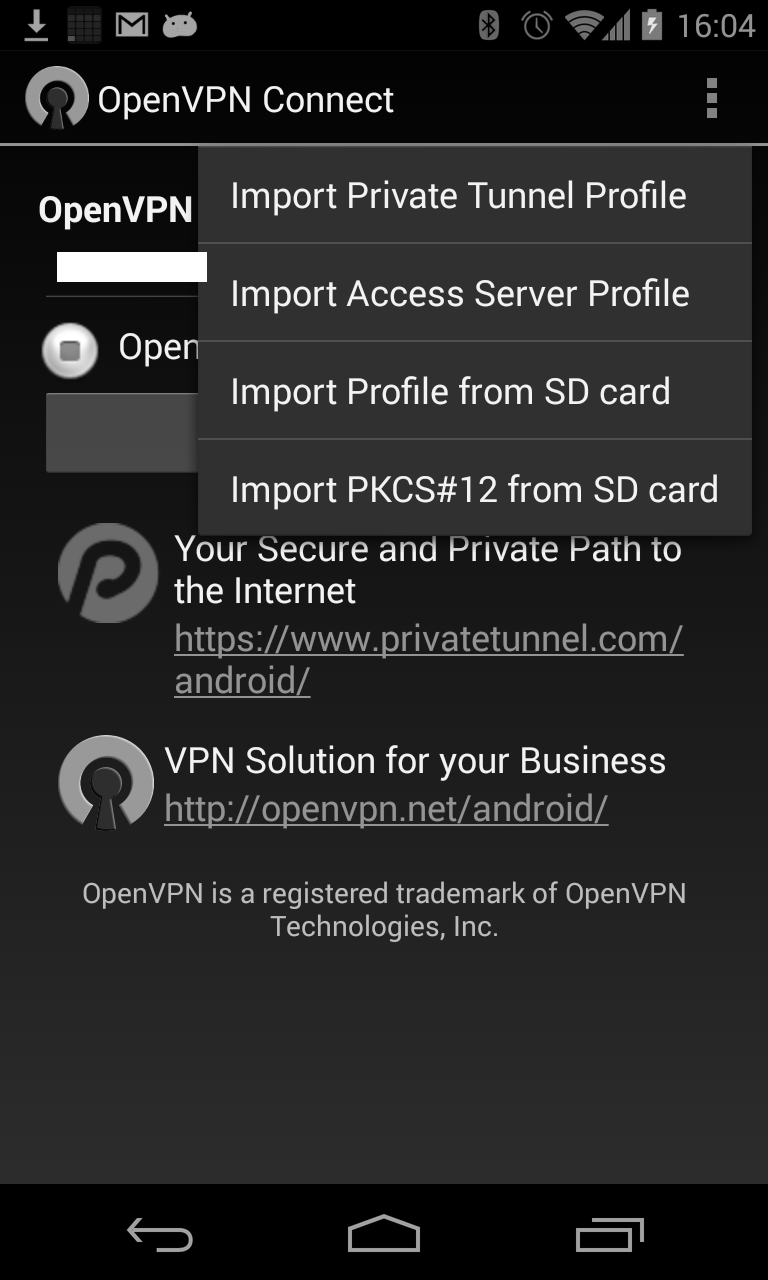
\includegraphics[width=0.3\hsize,bb=0 0 768 1280]{image201308/Screenshot_2013-08-17-16-04-31_mono.png}
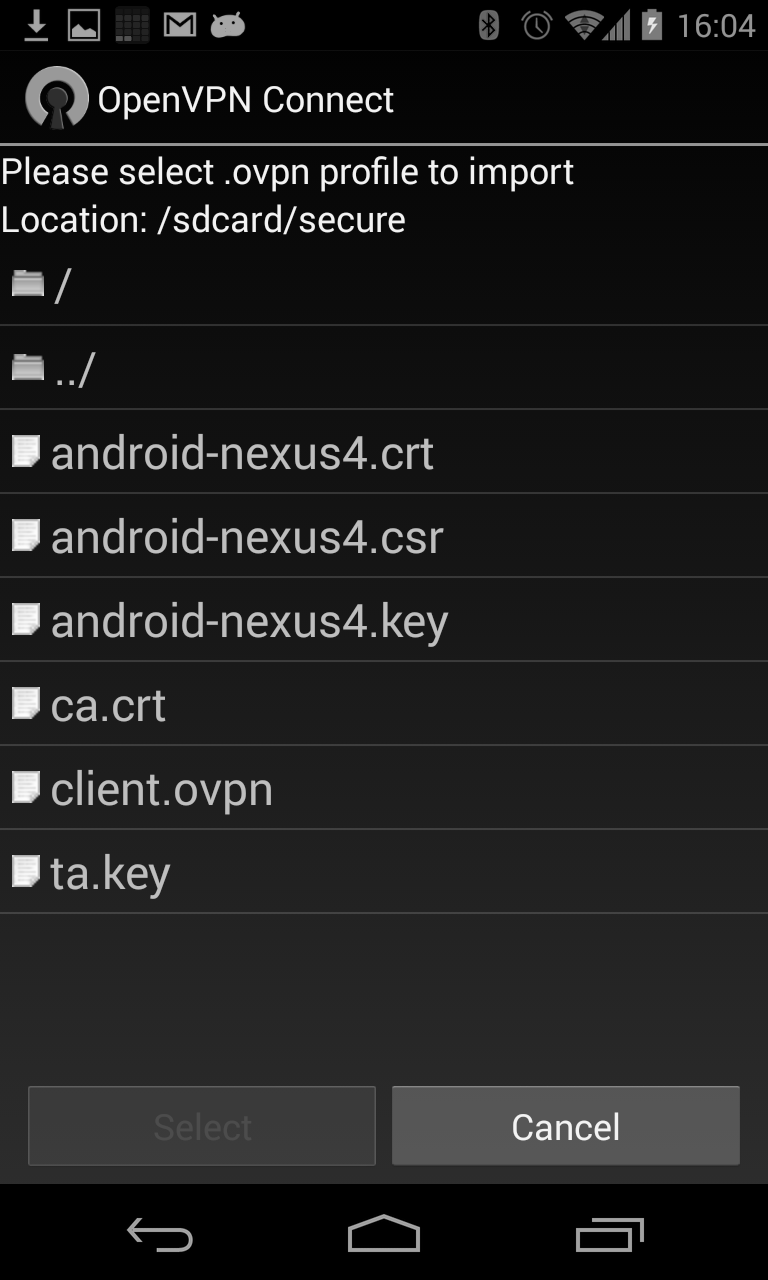
\includegraphics[width=0.3\hsize,bb=0 0 768 1280]{image201308/Screenshot_2013-08-17-16-04-43_mono.png}
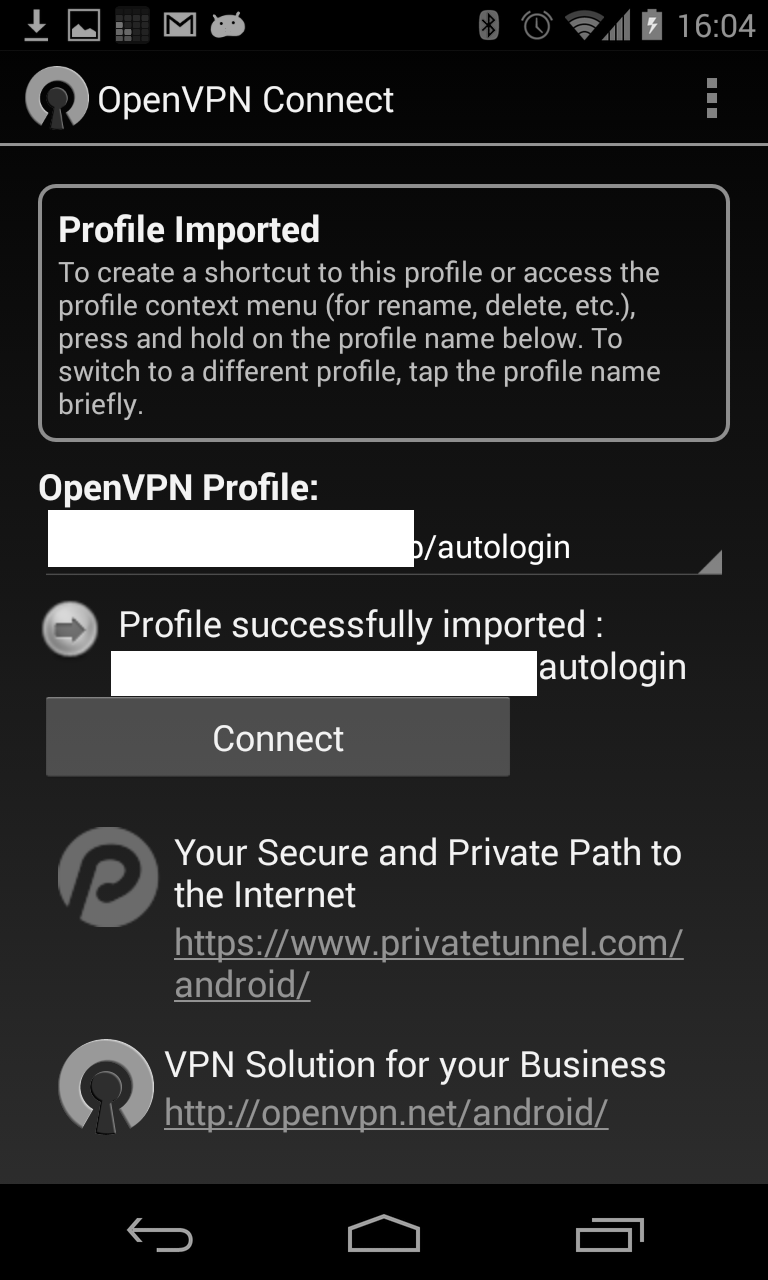
\includegraphics[width=0.3\hsize,bb=0 0 768 1280]{image201308/Screenshot_2013-08-17-16-04-54_mono.png}
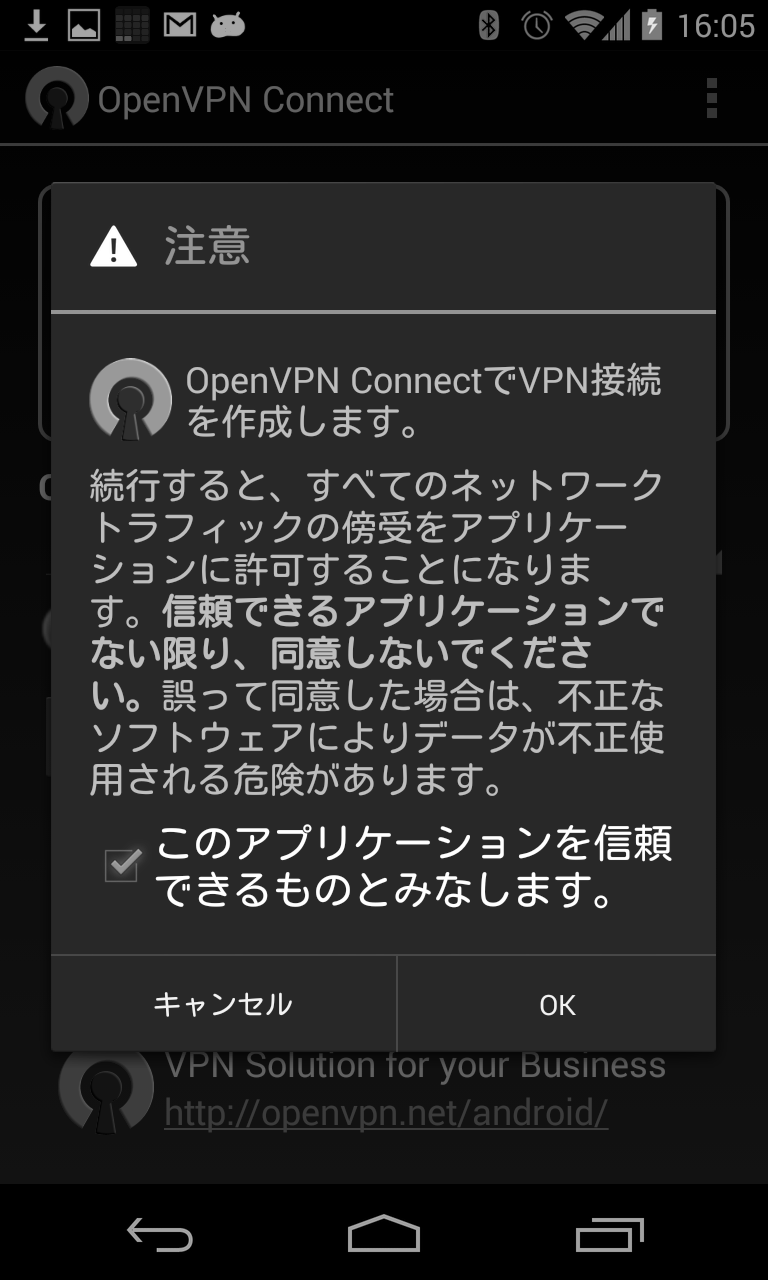
\includegraphics[width=0.3\hsize,bb=0 0 768 1280]{image201308/Screenshot_2013-08-17-16-05-07_mono.png}

インポートしたらsdcardからファイルを削除します。

\subsection{応用}

特に今回必要でなかったので設定しなかったのですが違う設定も可能なのでそれ
も紹介します。

ルーティングなどは openvpn サーバ側で設定すればクライアントに設定を配布
(push)してくれるようです。

\subsubsection{ローカルネットワークへのゲートウェイを設定したい}

redirect-private オプションでVPN経由でのルーティングを設定します。
たとえば、VPN経由のゲートウェイ(たとえば 10.0.0.1) 経由で 自宅のネット
ワーク(例えば 192.168.1.0/24) にアクセスできるようにしたいときに使えま
す。

\url{/usr/share/doc/openvpn/examples/sample-config-files/firewall.sh}に
iptablesの設定例が掲載されています。

\subsubsection{暗号化経路のためにすべてのパケットをVPN経由にしたい}

redirect-gateway オプションで指定できます。

公共の WiFi スポット経由での通信などが安心できない人向けのオプションです。
しかしDHCPの再リースやDNSの名前解決などもVPN経由になってしまうと困る場合
もあるので bypass-dhcp, bypass-dns オプションなどがあるようです。

\subsection{おわりに}

openvpn 2.3 でgitリポジトリの再編を行ったようで、
easy-rsaとかが分離されたっぽいです。

マニュアルを読んでいるとWindows 版の専用オプションとかが複雑にからみあっ
ていて実際どれをつかえばよいのか読み解きにくいです。最低限動かすまではそ
こまで難しくないのですがルーティングとかデフォルトゲートウェイを変更し
ようかと考え始めると考えることがいくつかあるようです。
しかし一般論で考えても、ネットワーク3つ以上を接続する場合のファイアウォー
ルとかルーターの設定はそれなりに複雑ですから、それを考えると妥当なのかも
しれませんね。

\subsubsection{ssh の各機能との比較}

開発者・運用者愛用のツールsshとどう違うのかとおもってみてみたのですが、
sshにも VPN 機能もあるので比較しにくいですね。ただ、通常の運用ではroot同
士でsshすることはあまりないかと思いますが、VPNを利用するにはrootでssh で
きる必要があるようです。

openvpnのメリットとしては openvpn には接続が切れた時を検出して再接続する
仕組みがあること、TCPだけでなくUDPも使えること、root 権限でsshログインを
許可しないでよいことなどがあげられると思います。

\begin{table}[H]
 \caption{ssh の機能の対応}
 \begin{tabular}{|c|c|c|}
 \hline
 \hline
 & sshオプション & 機能 \\
 \hline
 ポートフォワーディング &  -L, -R & 特定のローカルのTCPポート番号をリモートのポート番
	 号とマッピングする \\
 \hline
 プロキシ & -D & SOCKSに対応しているアプリケーションのプロキシを提供 \\
 \hline
 VPN & -w & IPレベルで相互に見えるよう仮想的にネットワークを構築する \\
 \hline
 \hline
 \end{tabular}
\end{table}


\begin{thebibliography}{0}
 \bibitem{openvpndebianwiki} \url{http://wiki.debian.org/OpenVPN}
 \bibitem{openvpnmanpage} openvpn(8) manpage
 \bibitem{openvpnreadmedebian} OpenVPN README.Debian \url{/usr/share/doc/openvpn/README.Debian.gz}
 \bibitem{openvpnnetcommunity} OpenVPN Community Software
	 \url{http://openvpn.net/index.php/open-source.html}
 \bibitem{rfc5246}
	 The Transport Layer Security (TLS) Protocol
	 Version 1.2
	 \url{https://tools.ietf.org/html/rfc5246}
\bibitem{openvpnconnectandroid} OpenVPN Connect Android app
	\url{https://play.google.com/store/apps/details?id=net.openvpn.openvpn}
\end{thebibliography}

%201311 tokyo
%-------------------------------------------------------------------------------
\dancersection{waylandを動かす}{野島 貴英}
%-------------------------------------------------------------------------------
\index{wayland}

\subsection{wayland}
 waylandとは、Kristian H\o{}gsbergさんが中心となって作っているディスプレイサーバーのプロトコルのことです。waylandプロトコルを扱えるディスプレイサーバーとしてwestonがあります。
\index{weston}

 従来からあるUnixで有名なディスプレイサーバーのプロトコルとしては、Xプロトコルがあり、Xプロトコルを扱えるディスプレイサーバーにXがあります。しかしながら、Xは1984年頃の設計から始まって、ずっとハードの進化にあわせてつぎはぎしてきたため、いろいろ実装と機能に無理が生じています。waylandは、Xに比べて、圧倒的に洗練された設計で、シンプルに、プロトコルとディスプレイサーバーを実現したものとなります\cite{real-wayland-X}。


\subsection{westonの動いている様子}

 westonの動いている様子を載せます。

\begin{minipage}{0.5\hsize}
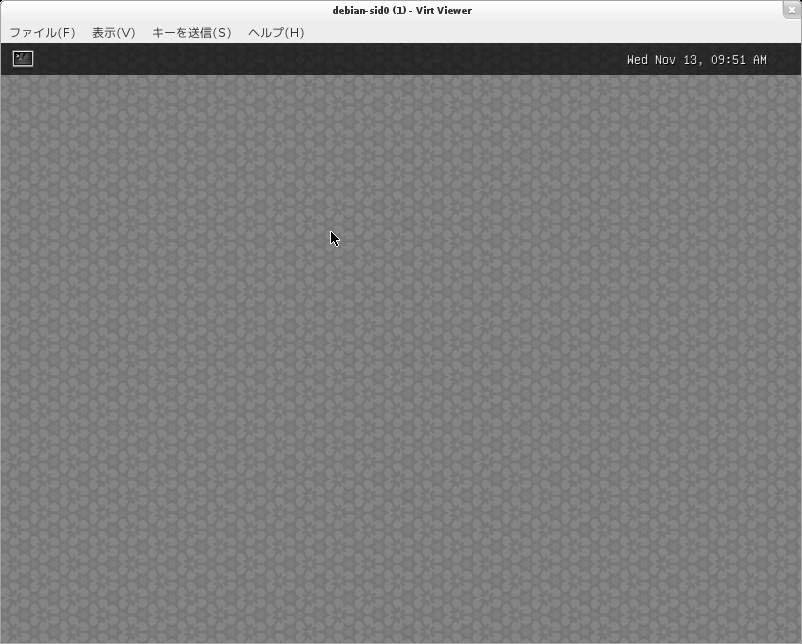
\includegraphics[width=0.8\hsize]{image201311/weston-1st-launch_mono.png}
\end{minipage}
\begin{minipage}{0.5\hsize}
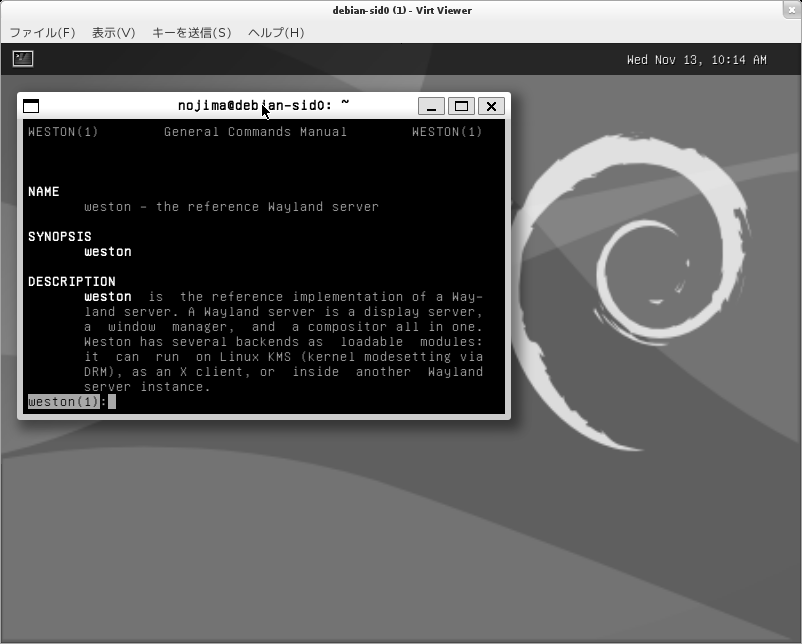
\includegraphics[width=0.8\hsize]{image201311/weston-2nd-launch_mono.png}
\end{minipage}

\subsection{westonの対応出力デバイス}

 westonの対応できる出力デバイスは表\ref{tab:debian-weston-backends}となります。

\begin{table}[ht]
\begin{center}
\begin{tabular}{|l|p{4cm}|p{4cm}|p{3cm}|l|}
\hline
項番&出力デバイス&バックエンド名&パッケージに搭載済&備考\\
\hline \hline
1& DRM/KMS & drm-backend.so & ○ & \\
2& FrameBuffer & fbdev-backend.so & ○ & \\
3& X & x11-backend.so & ○ & \\
4& Wayland & wayland-backend.so & ○ & \\
5& Headless & headless-backend.so & ○ & \\
5& Rassberry Pi & rpi-backend.so & × & \\
6& RDP & rdp-backend.so & × & \\
\hline
\end{tabular}
\label{tab:debian-weston-backends}
\caption{出力デバイスとwestonの対応状況}
\end{center}
\end{table}

\subsection{debianでのweston稼働のための下準備}
\label{sec:pre-requisite}
debianでwestonを動作させるには、以下の下準備が必要です。

\begin{description}
\item [Step 1.] westonの導入をします。
\begin{commandline}
# aptitude install weston
\end{commandline}
\item [Step 2.] systemdパッケージを導入するなどして、環境変数XDG\_RUNTIME\_DIRが設定されるようにします。
\begin{commandline}
# aptitude install systemd
\end{commandline}
\item [Step 3.] weston-launchにユーザを加え、ログインしなおします。
\begin{commandline}
# usermod -a -G weston-launch <your-login-id>
...重要:この後ログインしなおす...
\end{commandline}
\item [Step 4.] 環境変数XDG\_RUNTIME\_DIRが設定されているか確かめます。なお、何らかの理由で、systemdパッケージ付属のsystemd-logindが動作しない等の理由により、XDG\_RUNTIME\_DIRが設定されていないのであれば、export XDG\_RUNTIME\_DIR=/tmpなどして書き込みが可能なディレクトリを指定しておきます。
\begin{commandline}
[1] systemd-logindが無事動いている場合↓
$ env | fgrep XDG_RUNTIME_DIR
XDG_RUNTIME_DIR=/run/user/1000

[2] systemd-logindが何らかの理由で動作していない場合↓
$ env | fgrep XDG_RUNTIME_DIR
...なにも表示されない...
$ export XDG_RUNTIME_DIR=/tmp
\end{commandline}
%$
\end{description}

\subsection{その1:X上で動かしてみる}

一番簡単に動かせます。Xのターミナルソフト上で、

\begin{commandline}
$ weston
\end{commandline}
% $

とするだけで、x11-backend.soが読み込まれ、
westonの窓が開き、westonが動作を開始します。

停止する時は、westonを起動しているターミナルで、Ctrl-Cを押下します。

\subsubsection{X上で動かしてみる時の注意点}

何故か、手元のnvidia製グラフィクスカードにて、non-freeのnvidiaドライバを
使っていると、画面真っ黒のウィンドウが開いてしまいました。--use-pixmapを指定
してwestonを起動して、westonがEGL等のハードウェアアクセラレーションを
利用しないようにしても同様だったりします。一方で、intel製のグラフィクス
チップを載せているノートPC上では問題なく動作しました。

こちらの原因はまだつかめていません。

\subsection{その2:KMS/DRMで動かしてみる}

intelのグラフィックスチップが搭載されているPC(例:ノートPCとか)
であれば、linuxのKMS/DRMドライバで動作します。また、
AMD/Nvidiaのグラフィクスチップであれば、linuxのKMS/DRMドライバの
radeon/nouveauドライバで動作すると思われますが、自分は未評価です。
どなたかradeon/nouveauで動作した方がいらっしゃれば教えてください。

\begin{description}
\item [Step 1.] グラフィカルなログイン画面が出ているようであれば、こちらを停止させます。\\
例:gdm3が立ち上がっている場合の止め方
\begin{commandline}
Ctrl-Alt-F1等を押下してコンソールに切り替える
$ su
# service gdm3 stop
\end{commandline}
%$
\item [Step 2.] KMS/DRMドライバが有効であることを確かめます。
\begin{commandline}
$ lsmod | egrep '(i915|radeon|nouveau)'
...(i915/radeon/nouveauのどれかの文字列が出ればOK)...
\end{commandline}
%$
\item [Step 3] westonを動かします。
\begin{commandline}
$ weston-launch
\end{commandline}
%$
\end{description}

\subsubsection{KMS/DRM上で動かしてみる時の注意点}

 linuxのKMS/DRMドライバは、i915/radeon/nouveau以外は動作するかどうかは正直やってみないと分かりません。

 例えば、debianにて、仮想化技術のKVMではcirrusチップセット用のKMS/DRMドライバがvirt-viewerの元で使えるのですが、westonはegl側cirrus未対応によるエラーもしくは、Segfaultで落ちてしまうためどうにも動作しませんでした。こちらも原因が自分では正確につかめていません。

\subsection{その3.FrameBufferデバイス上で動かしてみる}

 linuxのFrameBufferデバイス上で動かしてみます。今のところ仮想化技術のKVM上で動かすのに便利です。ここでは、実際にKVMを使って動かします。

 なお、大変残念なことに、現在のdebian sidで導入できるwestonパッケージのバージョン1.3.0では、仮想端末制御に関するupstream側のバグのために、FrameBufferデバイスでは動作しません。幸い、こちらのバグが修正された、weston-1.3.1がリリースされましたので、ここでは、このバージョンを簡易的にdebianパッケージ化して導入します。

\begin{description}
\item [Step 1.]  westonを動かす対象のdebian sidをKVMを使ってインストールします。なお、KVMホストOS側のdebian機のbr0はインターネットに接続できるように設定されているものとします。br0のセットアップについて、詳しくは\cite{kde-devel-debian}を参照してください。
\begin{commandline}
# aptitude install libvirt-bin virtinst
# qemu-img create -f raw /var/lib/libvirt/images/debian-sid0 10G
# wget http://cdimage.debian.or.jp/7.2.0/multi-arch/iso-cd/debian-7.2.0-amd64-i386-netinst.iso
# virt-install --connect=qemu:///system -n debian-sid0 --ram 512  --cdrom /home/yours/debian-7.2.0-amd64-i386-netinst.iso \
  --disk /var/lib/libvirt/images/debian-sid0,bus=virtio,size=10,format=raw,cache=writeback \
  --bridge=br0,model=virtio --vnc --hvm --accelerate
\end{commandline}

 なお、インストールの際の設定は表\ref{tab:inst-settings}のとおりを仮定します。

\begin{table}[ht]
\begin{center}
\begin{tabular}{|l|p{5cm}|p{7cm}|l|}
\hline
項番&設定項目&指定内容&備考\\
\hline \hline
1&select a language& Japanese& \\
2&場所の選択&日本&\\
3&ネットワークの設定&手動設定。 IP:192.168.0.2, Netmask:255.255.255.0, Gateway:192.168.0.1, Host名:debian-sid0& \\
4&パッケージマネージャの設定&ミラー:日本,ミラーサイト:ftp.jp.debian.org, HTTPプロキシ:空欄&\\
5&ソフトウェアの選択&SSHサーバー、標準システムユーティリティのみ選択。あとはすべて解除。& \\
\hline
\end{tabular}
\caption{\label{tab:inst-settings}インストーラで選択する項目}
\end{center}
\end{table}

\item [Step 2.] インストール完了したら、すぐにdebian sidへアップグレードします。

\begin{commandline}
debian-sid0にログインの後、
debian-sid0 $ su
debian-sid0 # cat > /etc/apt/sources.list
deb http://ftp.jp.debian.org/debian/ sid main contrib non-free
deb-src http://ftp.jp.debian.org/debian/ sid main contrib non-free
<ctrl+d>を押下
debian-sid0 # aptitude update;aptitude full-upgrade;aptitude clean
\end{commandline}
%$

\item [Step 3.] weston-1.3.1-1パッケージを作って導入します。

\begin{commandline}
debian-sid0 # aptitude build-dep weston/sid
debian-sid0 # aptitude install libxcb-composite0-dev fakeroot
debian-sid0 # exit
debian-sid0 $ mkdir weston weston-work
debian-sid0 $ cd weston
debian-sid0 $ apt-get source weston/sid
debian-sid0 $ cd ../weston-work
debian-sid0 $ wget -O weston_1.3.1.orig.tar.gz \
  http://cgit.freedesktop.org/wayland/weston/snapshot/weston-1.3.1.tar.gz
debian-sid0 $ tar xzf weston_1.3.1.orig.tar.gz
debian-sid0 $ cd weston-1.3.1
debian-sid0 $ tar xzf ../../weston/weston_1.3.0-1.debian.tar.gz
debian-sid0 $ cd debian;
debian-sid0 $ patch -p1 <<__HERE
--- debian.org/changelog        2013-10-11 20:04:50.000000000 +0900
+++ debian/changelog    2013-11-12 14:48:36.219299000 +0900
@@ -1,3 +1,9 @@
+weston (1.3.1-1) unstable; urgency=low
+
+  * update to upstream
+
+ -- your name <foo@bar.com>  Fri, 11 Nov 2013 12:34:56 +0900
+
 weston (1.3.0-1) unstable; urgency=low

   [ Sven Joachim ]
diff -ru debian.org/control debian/control
--- debian.org/control  2013-10-11 19:58:17.000000000 +0900
+++ debian/control      2013-11-12 14:49:32.347299000 +0900
@@ -35,6 +35,7 @@
  libpam0g-dev,
  libvpx-dev,
  libsystemd-login-dev,
+ libxcb-composite0-dev,
 Standards-Version: 3.9.4
 Homepage: http://wayland.freedesktop.org/
 Vcs-Git: git://anonscm.debian.org/pkg-xorg/wayland/weston
__HERE
debian-sid0 $ cd ..
debian-sid0 $ env DEB_BUILD_OPTIONS='noopt nostrip' \
   dpkg-buildpackage -rfakeroot -us -uc 2>&1 | tee ../build.log
debian-sid0 $ cd ..
debian-sid0 $ su
debian-sid0 # dpkg -i ./weston_1.3.1-1_amd64.deb
\end{commandline}

\item [Step 3.]  \ref{sec:pre-requisite}章のStep 2.〜Step 4.に記載の下準備をしておきます。(Step 1.は先ほど構築したwestonパッケージが導入済みですので不要です)


\item [Step 4.] FrameBufferのセットアップをします。なおwestonを動かすためには、color depthは24bitでなければなりません。
\begin{commandline}
debian-sid0 # aptitude install fbset
debian-sid0 # modprobe cirrusfb
debian-sid0 # fbset -g 800 600 800 600 24
\end{commandline}

\item [Step 5.] 一般ユーザになり、westonを起動します。
\begin{commandline}
debian-sid0 # exit
debian-sid0 $ weston-launch -- --backend=fbdev-backend.so --log=weston.log
\end{commandline}
%$
\end{description}

\subsection{westonのカスタマイズ}

 westonはデフォルトのままだと少し寂しい画面なので、ちょっとカスタマイズしてみます。カスタマイズは$HOME/.config/weston.iniにいろいろ記載すると、いろいろとカスタマイズできます。ここでは壁紙を入れ、ウィンドウポップアップがアニメーションするようなカスタマイズをしてみます。
\begin{commandline}
$ cat >.config/weston.ini <<__HERE
[shell]
background-image=/usr/share/images/desktop-base/spacefun-grub.png
background-type=tile
locking=true
animation=zoom
binding-modifier=ctrl

[launcher]
icon=/usr/share/weston/terminal.png
path=/usr/bin/weston-terminal
__HERE
\end{commandline}
%$

\subsection{westonの構造}

 図\ref{fig:wayland-internal}にwaylandアプリケーションとwestonの構造を載せます。

\begin{figure}[H]
\begin{center}
 \includegraphics[width=0.8\hsize] {image201311/wayland-internal-schema.eps}
 \caption{waylandアプリケーションとweston}
\label{fig:wayland-internal}
\end{center}
\end{figure}

 特徴として、
\begin{itemize}
\item 基本的にアプリケーション側も含めて、ローカルシステムで描画を行うことを前提にした作りになっています。
\item cairo/mesa/xkbcommon等を最大限利用して、weston自体は非常にシンプルな設計になっています。
\item プロセスのユーザ権限を制限するため、weston-lanchにはroot権限が最低限必要な部分のみの操作を、westonは一般ユーザでの権限による動作をするように、権限が分割されています。なお、現在の実装ではweston-launchは操作・オープン済みの端末のFileDiscriptorと、デバイスファイルのFile Descriptor、weston-launchへのシグナルを、westonの求めに応じて引き渡す機能が実装されています。
\end{itemize}
\subsection{その他}

 debianで利用できるweston/waylandにはちょっとしたクセがあります。

 \begin{itemize}
\item Xwaylandが動作しません。これはwestonが起動するXにwayland用のI/Fを搭載するパッチが摘要されていなければならない(X起動時に-waylandオプションが使えなければならない)のですが、こちらは未だXのパッケージに含められていない為となります。なお、2013/10頃にこちらのdebianパッケージ用のパッチがdebian-xのMLに流れていました。
\item gtk等の有名なツールキットはwayland未対応の状態です。
 \end{itemize}

\subsection{おわりに}

 次期ディスプレーサーバーになるかもしれないwestonとwaylandについて、いろいろ試してみました。プログラム本体は非常に小さいプログラムですし、発展途上ですので、いじってみようという方は、今ならたやすく改造/解析し放題の旬な時です。Hackの対象にぜひ。

\begin{thebibliography}{0}
  \bibitem{real-wayland-X}
    {\footnotesize{
       Daniel Stone,``The real story behind Wayland and X'',linux.conf.au 2013,
       \url{http://people.freedesktop.org/~daniels/lca2013-wayland-x11.pdf},
       \url{http://www.youtube.com/watch?v=RIctzAQOe44}
       }}
  \bibitem{kde-devel-debian}
    {\footnotesize{
       野島 貴英,「Debian開発者のKDE環境あれこれ」,第85回東京エリアDebian勉強会資料,
       \url{http://tokyodebian.alioth.debian.org/pdf/debianmeetingresume201202.pdf}
       }}
\end{thebibliography}

%201307 tokyo
%-------------------------------------------------------------------------------
\dancersection{月刊Debhelper dh\_strip}{野島 貴英}
%-------------------------------------------------------------------------------
\index{dh\_strip}

\subsection{今月のコマンド}

 今月はdh\_stripを取り上げます。紙面の都合でdh\_stripの1コマンドの
紹介に今回はとどめておきます。

\subsection{dh\_strip}

 dh\_stripコマンドは、 ``debian/tmp/'' 等のビルドディレクトリ以下を再帰的に
探し回り、ビルドしたばかりの実行ファイルのバイナリ、共有ライブラリのバイナリ、静的ライブラリのバイナリを見付けると、片っ端からバイナリに含まれているデバッグシンボルを取り除いてくれます。

 また、別途コマンドラインオプションを指定すると、取り除いたデバッグシンボルを別ファイルに取り置きます。このため、dh\_stripコマンドは*-dbgパッケージ作成の時に重要な役割を持ちます。

\subsubsection{すでに発表済みの件}

 実は、dh\_stripの*-dbgパッケージを作成する為の動作については、大統一Debian 2012のセッションである「debug.debian.net」\cite{debug-debian-net}のプレゼン資料に詳しいので、こちらを参照してください。

 また、*-dbgパッケージを使って実際にデバッグをしてみる件については、大統一Debian 2013のセッションである「gdb+python拡張を使ったデバッグ手法」\cite{gdb-python-debug2}に紹介していますので、こちらも参照ください。

 ここでは、これらの発表で扱わなかった件を重点的に記載します。

\subsubsection{debug/*.so,lib*\_g.aファイルの扱い}

 dh\_stripコマンドは、元々デバッグ用途として用意されているdebug/*.soファイルや、
lib*\_g.aファイルについては、何も処理を行いません。

\subsubsection{コマンドラインオプションと動作}

 dh\_stripコマンドは表\ref{tab:dh-strip-opt}のコマンドラインオプションを解釈します。

\begin{table}[ht]
\begin{center}
\small
\begin{tabular}{|p{8em}|p{35em}|}
\hline
オプション名&動作 \\ \hline \hline
man debhelper記載のオプション & こちらは全debhelperに共通のオプションです。動作はman debhelperに記載されていたり、以前の月刊debhelperで説明されているとおりとなりますので、ここでは割愛します。 \\ \hline
-Xitem, --exclude=item & itemで指定されるファイル名を持つバイナリを処理の対象から外します。複数のファイルを指定したい場合は、繰り返し指定すると指定できます。例: dh\_strip -Xfile1 -Xfile2 \\ \hline
--dbg-package=package & *-dbgパッケージを作る際に、デバッグシンボルを格納するパッケージ名を指定する為に利用します。通常、*-dbgパッケージを作る場合は、こちらのオプションを利用する事となります。なお、ソースパッケージにあるdebian/compatで指定されるCOMPATIBILITY LEVELで振る舞いが異なります(後述)。\\ \hline
-k & 分離したデバッグシンボルをバイナリパッケージに含める場合にこちらのオプションを利用します。この場合、出来上がったパッケージにはバイナリの他に、分離したデバッグシンボルも/usr/lib/debug/以下に含まれる形で収録されます。--dbg-packageが同時に指定されると、--dbg-packageの指定の方が優先されます。\\ \hline
\end{tabular}
\caption{dh\_stripコマンドラインオプション}
\label{tab:dh-strip-opt}
\end{center}
\end{table}

\subsubsection{COMPATIBILITY LEVELでの動作の違い}

 dh\_stripはソースパッケージに含まれるdebian/compatで指定される
COMPATIBILITY LEVELにより、振る舞いが変わります。

 --dbg-packageオプション指定時の振る舞いの違いは表\ref{tab:dh-strip-comp-level}に、
また、-k/--dbg-packageオプション指定時に生成されるデバッグシンボルファイルの違いについて表\ref{tab:debugsym-file-difference-comp-level}に、記載します。

\begin{table}[ht]
\begin{center}
\small
\begin{tabular}{|p{8em}|p{35em}|}
\hline
COMPATIBILITY LEVEL &--dbg-package指定時の動作 \\ \hline \hline
4以下 & ``dh\_strip --dbg-package=xxxx --dbg-package=yyyy''のように--dbg-packageを複数指定する事が出来ます。ここで、こちらで指定した名前(xxxxや、yyyy)に合致するパッケージを処理する際、''パッケージ名-dbg''というパッケージ名を*-dbgパッケージのパッケージ名として自動的に利用します。また、ソースパッケージに含まれるdebian/controlには、これら*-dbgパッケージの為の記述は不要となります。\\ \hline
5以上 & --dbg-packageは1つ指定するのが原則となります。もし複数指定した場合は、最初に指定された内容のみ利用されます。また、--dbg-package=xxxxxとすると、デバッグシンボルを格納するパッケージ名として、xxxxxがそのまま使われます。例えば、libfooパッケージと、fooパッケージを構築し、これらパッケージに含まれているバイナリのデバッグシンボルをfoo-dbgパッケージに全部入れるには、--dbg-package=foo-dbgと指定します。また、
ソースパッケージに含まれるdebian/controlには、生成予定の*-dbgパッケージの為の記述は必須となり、万一記載されていない場合はエラーとして扱われ、この場合はdh\_stripはエラーを表示して終了します。\\ \hline
\end{tabular}
\caption{COMPATIBILITY LEVELと--dbg-packageオプションの振る舞いの違い}
\label{tab:dh-strip-comp-level}
\end{center}
\end{table}

\begin{table}[ht]
\begin{center}
\small
\begin{tabular}{|p{8em}|p{35em}|}
\hline
COMPATIBILITY LEVEL &-k/--dbg-package指定時のデバッグシンボルファイルの違い \\ \hline \hline
8以下 & ``/usr/lib/debug/+バイナリのインストール先パス/+バイナリファイル名''に格納されるようにデバッグシンボルファイルが生成されます。また、デバッグに関する情報はコンパイラが生成したままの形で保存されるため、デバッグシンボルファイルのサイズは大きくなりがちです。\\ \hline
9以上 & バイナリがBuildID\cite{gdb-python-debug2}を含んでいる場合は、``/usr/lib/debug/.build-id/BuildIDの上位2桁/+BuildIDの残りの桁+.debug''に格納されるようにデバッグシンボルファイルが生成されます。BuildIDを含んでいなければCOMPATIBILITY LEVEL 8以下と同様のファイル名となります。また、BuildIDの有無にかかわらず、デバッグに関する情報はzlibにより圧縮されて格納されます。そのため、デバッグシンボルファイルのサイズはできるだけ小さくなるようになっています。\\ \hline
\end{tabular}
\caption{COMPATIBILITY LEVELと-k/--dbg-packageオプションの振る舞いの違い}
\label{tab:debugsym-file-difference-comp-level}
\end{center}
\end{table}

\subsubsection{デバッグシンボル}

 dh\_stripで取り分けられるデバッグシンボルは、elfバイナリベースのシステム\footnote{お馴染みのi386/amd64用linuxの場合等}であれば、DWARF\cite{dwarf-spec}をベースとした形式のファイルとなります。
\index{dwarf}

 ここでDWARFは、コンパイラを用いてCPUの命令に直接変換するようなコンパイル言語(C/C++等)を用いて作成したバイナリを対象として、ソースレベルのデバッグを行う場合に必要な/便利な情報を格納する為に作られた、よくできたフォーマットです。元々はSystem V用のデバッガであるsdbの為にBell研で開発されたフォーマットがベースとのことです\footnote{Bell研とか、System Vとか、今ではもう完全にオッサンホイホイな用語となってしまいました...}。DWARFは、''Debugging With Attributed Record Formats''の略とのことです。

 図\ref{fig:dwarf-vs-elf-schema}にバイナリと、デバッグシンボルの中身を
簡単に図示します。

\begin{figure}[h]
\begin{center}
\includegraphics[width=0.8\hsize]{image201307/dwarf-elf-schema.eps}
 \caption{バイナリと、デバッグシンボルの中身}
 \label{fig:dwarf-vs-elf-schema}
\end{center}
\end{figure}

\subsubsection{デバッグシンボルファイルの情報を覗いてみる}

 実はバイナリや、デバッグシンボルの中身を見る方法は知っておくと、
いろいろデバッグ等で役立つ場面が多いです。以下に簡単に参照する方法を載せます。

 まず、バイナリにはどんなヘッダ情報とセクションが入っているかのサマリを
掌握してみます。

\begin{commandline}
$ sudo aptitude install binutils
$ readelf -e /usr/bin/gst-launch
ELFヘッダ
   マジック:  7f 45 4c 46 02 01 01 00 00 00 00 00 00 00 00 00
  ...中略...
セクションヘッダ:
  [番] 名前              タイプ           アドレス          オフセット
       サイズ            EntSize          フラグ Link  情報  整列
  [ 0]                   NULL             0000000000000000  00000000
       0000000000000000  0000000000000000           0     0     0
  [ 1] .interp           PROGBITS         0000000000400238  00000238
       000000000000001c  0000000000000000   A       0     0     1
...中略...
  [27] .gnu_debuglink    PROGBITS         0000000000000000  00003240
       0000000000000034  0000000000000000           0     0     1
  [28] .shstrtab         STRTAB           0000000000000000  00003274
       00000000000000fe  0000000000000000           0     0     1
...中略...
\end{commandline}

 次にどんなデバッグシンボルファイルが使われる予定かを見てみます。

\begin{commandline}
$ readelf -x .gnu_debuglink /usr/bin/gst-launch
セクション '.gnu_debuglink' の 十六進数ダンプ:
  0x00000000 34326462 34373631 31386162 32623831 42db476118ab2b81
  0x00000010 30343161 63643830 65343565 38396534 041acd80e45e89e4
  0x00000020 32383965 61322e64 65627567 00000000 289ea2.debug....
  0x00000030 dbf8060d                            ....
$
\end{commandline}

 デバッグシンボルのファイル名の形式から、COMPATIBILITY LEVEL 9のソース
パッケージで構築されたデバッグシンボルファイルである事がわかります。
このため、BuildIDから、/usr/lib/debug/.build-id/9b/42db476118ab2b81041acd80e45e89e4289ea2.debugがデバッグシンボル
のファイルとなります。

 次にデバッグシンボルファイルから、ビルド時のディレクトリ位置を求めてみます。

\begin{commandline}
$ aptitutde install libgstreamer0.10-0-dbg
$ readelf -wi /usr/lib/debug/.build-id/9b/42db476118ab2b81041acd80e45e89e4289ea2.debug | lv
.debug_info セクションの内容:

  コンパイル単位 @ オフセット 0x0:
   長さ:        0x1b3b (32-bit)
   バージョン:    2
   Abbrev Offset: 0x0
   ポインタサイズ:8
 <0><b>: 省略番号: 1 (DW_TAG_compile_unit)
    <c>   DW_AT_producer    : (間接文字列、オフセット: 0x442): GNU C 4.7.2

    <10>   DW_AT_language    : 1        (ANSI C)
    <11>   DW_AT_name        : (間接文字列、オフセット: 0x57a): gst-run.c

    <15>   DW_AT_comp_dir    : (間接文字列、オフセット: 0x36b): /tmp/buildd/gstr
eamer0.10-0.10.36/tools
 ...中略...
\end{commandline}
%$

 .debug\_infoセクションに定義されている、DW\_TAG\_compile\_unitの結果から、 \\
ディレクトリ/tmp/buildd/gstreamer0.10-0.10.36/toolsに配置されている
gst-run.cがコンパイルされている事がわかります。

 では、この結果を元に、gdbのset substitute-pathを使ってgdbでソースの
閲覧をやってみます\footnote{なお、本方法は、2013年大統一Debian勉強会\cite{gdb-python-debug2}の当時では、自分がまだ見つけていなかった方法でして...これでgdbのdirコマンドを使わなくて済み、今後は*-dbgパッケージを導入するだけで便利にソースの閲覧できるようになります。}。

\begin{commandline}
$ pwd
/home/yours/src/gstreamer/
$ apt-get source gstreamer0.10-tools/sid
$ gdb --args /usr/bin/gst-launch
...中略...
Reading symbols from /usr/bin/gst-launch...Reading symbols from
/usr/lib/debug/.build-id/9b/42db476118ab2b81041acd80e45e89e
4289ea2.debug...done.
(gdb) set substitute-path /tmp/buildd/ /home/yours/src/gstreamer/
(gdb) b main
(gdb) run
(gdb) l
313	  return candidates;
314	}
315
316	int
317	main (int argc, char **argv)
318	{
319	  GHashTable *candidates;
320	  gchar *dir;
\end{commandline}
%$

無事ソース閲覧ができています。

\subsection{おわりに}

 今回は、dh\_stripコマンドをネタに、デバッグシンボルファイル
の中を覗き、その結果を元に最後はgdbでソース閲覧ができるようになる
までをやってみました。

 また、dh\_stripの周辺技術を見てみると、ソースコードのデバッグができるように
なる為に、とても多くの人の成果物を活用していることが実感できました。

\begin{thebibliography}{0}
    \bibitem{debug-debian-net}
      {\footnotesize{
          2012年大統一Debian勉強会「debug.debian.net」,
          \url{http://gum.debian.or.jp/2012/}
        }}

    \bibitem{gdb-python-debug2}
      {\footnotesize{
          2013年大統一Debian勉強会「gdb+python拡張を使ったデバッグ手法」,
          \url{http://gum.debian.or.jp/2013/slide_data_list}
        }}
    \bibitem{dwarf-spec}
      {\footnotesize{
          The DWARF Debugging Standard,
          \url{http://www.dwarfstd.org/Home.php}
        }}

\end{thebibliography}

%201308 tokyo
%-------------------------------------------------------------------------------
\dancersection{Debian勉強会の資料のePUB化を試みた}{まえだこうへい}
%-------------------------------------------------------------------------------
\index{epub}
\index{latex}
\index{pdf}

\subsection{ePUB化の動機}

最近はかなりスマートフォンやタブレットが普及し、それ以外のeBook readerも東京周辺の電車内でも見かけるようになりました。Debian勉強会の参加者もそれらのデバイスを持っている人も今までちらほら見かけています。Debian勉強会の事前配布資料や年2回の「あんどきゅめんてっどでびあん\footnote{現在名前は違いますが、これが一番通りは良いと思うのでこのまま表記します。}」をそれらのデバイスで読む機会も増えているのではないでしょうか。\footnote{勉強会当日参加者に質問したらほとんどいないという結果でした。}

ところで、Debian勉強会の資料はLaTeXをソースとしてPDFとして配布されています。PDFは印刷物と同じレイアウトになるので、本勉強会のように印刷した資料を頒布する上では最適です。しかし、画面で閲覧するのには向いていないと思いませんか。その一番の理由は多くのPDFリーダーは、画面に最適な大きさで自動的にリサイズされないためだと考えています。\footnote{ここでは印刷物に比べて読みにくい、という観点では論じません。}読みたい部分を拡大表示することはできますが、画面サイズに合わせた文字が巻き返しはされず、画面外にでた続きの文章は横方向にスクロールしなくてはなりません。これは面倒です。

そこでePUBです。O'Reilly, 達人出版会から出版されているEbookの多くはePUBが採用されているので、これらを既に購入、読んでいる人もいるでしょう。ページあたりの構成が画面サイズに最適化され、かつ、フォントサイズの変更でもページが自動的にリサイズされるので、これらのデバイスで読むのにはうってつけでしょう。

今回はDebian勉強会の資料を、LaTeXのソースコードには極力手を加えずに\footnote{PDFは今まで通り印刷物用に必要なので。}ePUBを生成できないか検証しました。

\subsection{LaTeXからのePUB生成の方法}

\LaTeX から ePUBを生成するにはいくかの方法があります。取りうる手段としては4パターンです。

\begin{itemize}
  \item[1)] \LaTeX から直接 ePUBを生成する
  \item[2)] a. TeX もしくは b. DVIから, XMLもしくはHTMLを生成し、2)-2. ePUBに変換する
  \item[3)] PDFからePUBに変換する
\end{itemize}

\begin{figure}[H]
\begin{center}
  \includegraphics[width=0.7\hsize]{image201308/latex-epub.eps}
 \caption{LaTeXからePUBへの変換}
 \label{fig:convert-latex-to-epub}
\end{center}
\end{figure}

これらを行うためのツールについて検証しました。

\subsection{検証結果}

基本的にDebianパッケージになっているツールで検証を行いました。
対象は次の2つのファイルです。

\begin{enumerate}
  \item Debian勉強会の資料 (debianmeetingresume2013007.tex)
  \item latex2epubのサンプル \TeX ファイル (sample.tex)
\end{enumerate}

その結果は下記の通りです。

{\small
\begin{tabular}{|c|c|c|c|c|c}
\hline
パターン & ツール名 & 入力 & 出力 & \multicolumn{2}{|c|}{結果} \\ \cline{1-4}
 & & & & Debian勉強会の資料 & latex2pub のサンプル \\
\hline
1) & Pandoc & \LaTeX & ePUB & NG & OK \\
1) & latex2epub & \LaTeX & ePUB & NG & OK \\
2)-a & \LaTeX ML & \LaTeX & XML & NG & OK \\
2)-b & \TeX4ht & DVI & HTML & NG & NG \\
2)-b & htplatex(\TeX4ht) & \TeX & HTML & OK & NG \\
3) & Pandoc & HTML & ePUB & OK & N/A \\
4) & Calibre & PDF & ePUB & OK & OK \\
\hline
\end{tabular}
}


Debian勉強会の資料と、latex2epupのサンプル(以後、サンプルファイル)とで結果に大きな差がありますが、エラーメッセージを見る限りでは、その主な原因は使用しているdocumentclassの違いと、マクロの有無によるものではないかと考えられます。が、ここはあまり深堀できていません。

\subsection{変換できたケースでの課題}

Debian勉強会の資料で変換できたケースでの課題を挙げます。

\subsubsection{htplatex \& pandoc}

現状では次の問題がありますが、今回検証した中では一番まともに読める形で変換することができました。

\begin{itemize}
  \item tabularがtableに変換されず、表にならない
  \item 表紙の画像が追加されない
  \item あんどきゅめんてっどでびあん夏号、冬号をそれが含まれる月よりも先に変換すると、その中で使われている画像がhtmlディレクトリにコピーされず、ファイルが無いためpandoc実行時に失敗する
  \item \TeX4htでHTML変換時に自動生成される画像のファイル名が異なり、同じくpandoc実行時に失敗する月もある(2013年4月など)
  \item PDFを生成する場合(= makeを実行する場合)、htplatexが依存するパッケージ dvi2ps-fontdata-a2n をアンインストールする必要がある。これをアンインストールしないと、dvipdfmxでのDVIからPDF変換時に、"\texttt{** ERROR ** Virtual fonts nested too deeply}"というエラーが出て失敗する
\end{itemize}

なお、\TeX4ht は、実は上川さんが既に通った道でした。\footnote{\url{http://lists.debian.or.jp/debian-users/200708/msg00110.html}}
Debian勉強会の資料のリポジトリの中に、htplatexというシェルスクリプトがあります。
このスクリプトはDebian勉強会の資料の \LaTeX のファイルを \TeX4htを使ってHTML化するものです。

このスクリプトを使った手順は次のとおりです。

このスクリプトの2行目に使い方、3行目に依存パッケージのインストールについて記載されています。
まず、必要なパッケージをインストールします。

\begin{commandline}
$ apt-get install dvi2ps-fontdata-a2n dvi2dvi dvipng
\end{commandline}

次にスクリプトを実行します。

\begin{commandline}
$ ./htplatex debianmeetingresume200708.tex jp,2,sections+
\end{commandline}

すると、./html/ディレクトリ下に \LaTeX から変換されたHTMLが生成されます。
これをpandocを使ってePUBに変更します。

\begin{commandline}
$ cd html
$ pandoc -o debianmeetingresume200708.epub debianmeetingresume200708*.html
\end{commandline}

なお、このスクリプトは実行時に、"\texttt{-e}"オプションをつけることで、ePUBを生成することができるようにしました。

\begin{commandline}
$ ./htplatex -e debianmeetingresume200708.tex jp,2,sections+
\end{commandline}

変更内容は下記リンク先をご参照下さい。

\url{http://goo.gl/2KshN0}

\subsubsection{calibre}

calibreでは次の課題があります。

\begin{itemize}
  \item 目次のレイアウトが崩れる
  \item デフォルトでは行間が広すぎる
  \item 図が表示されない場合もある
  \item tabularが表として表示されない
\end{itemize}
変換時に、"ヒューリスティック処理を有効にする"にチェックを入れ、"外観"の"段落の間の間隔を削除する"にチェックを入れると、一部は多少改善されます。

\subsection{結論}
現時点では、 \LaTeX からのePUB生成は、不完全ながらも一応可能なようです。どれを選択するかはユーザ次第ではありますが、
いずれにしても更に使えるようにするには、各ツールでのパターンマッチングの機能を充実させる必要があるのではないかと思います。

しかし、iPad miniくらいの大きさのデバイスでは、Debian勉強会の資料のPDF版でもギリギリ拡大させなくても読めてしまいます。
ですので、PDFをそのまま読むのが一番読みやすい、という状況を解消できるようにしていくのが、我々の今後のアクションとなるに違いないでしょう。

\subsection{追記}

勉強会当日のディスカッションの結論としては、リフロー可能なPDFリーダをフリーソフトウェアとして作るのが正だろう、という話に落ち着きました。ちなみに自由ではないソフトウェアとしては、Adobe Readerならリフロー可能なようです。\url{http://code.kzakza.com/2013/05/pdf_reflow/}


\begin{thebibliography}{0}
 \bibitem{whatsthebesttextohtmlepubconverter} What’s the best \TeX-to-HTML or \TeX-to-ePUB converter?
   \url{http://boolesrings.org/krautzberger/2013/01/05/whats-the-best-tex-to-html-or-tex-to-epub-converter/}
 \bibitem{toolsforcovertinglatextoxml} Tools for Converting \LaTeX to XML
   \url{http://jblevins.org/log/xml-tools}
 \bibitem{pandoc} Pandoc \url{http://johnmacfarlane.net/pandoc/README.html}
 \bibitem{lxir} LXir \url{http://www.lxir-latex.org/}
 \bibitem{hermes} Hermes \url{http://hermes.roua.org/}
 \bibitem{texwiki} \TeX Wiki \url{http://oku.edu.mie-u.ac.jp/~okumura/texwiki/}
 \bibitem{tex4ht} \LaTeX をウエッブに載せよう
   \url{http://osksn2.hep.sci.osaka-u.ac.jp/~naga/miscellaneous/tex4ht/tex4ht-howto.html}
 \bibitem{latex2epub} \LaTeX2EPUB \url{http://kmuto.jp/d/index.cgi/computer/latex2epub.htm}
\end{thebibliography}

%-------------------------------------------------------------------------------
\dancersection{Debian Trivia Quiz}{上川 純一、岩松 信洋}
%-------------------------------------------------------------------------------

ところで、みなさん Debian 関連の話題においついていますか?Debian関連の話
題はメーリングリストをよんでいると追跡できます。ただよんでいるだけではは
りあいがないので、理解度のテストをします。特に一人だけでは意味がわからな
いところもあるかも知れません。みんなで一緒に読んでみましょう。

今回の出題範囲は\url{debian-devel-announce@lists.debian.org} や \url{debian-devel@lists.debian.org}に投稿された
内容とDebian Project Newsからです。

\begin{multicols}{2}
%; whizzy-master ../debianmeetingresume201211.tex
% 以上の設定をしているため、このファイルで M-x whizzytex すると、whizzytexが利用できます。
%

\santaku
{Stefano Zacchiroli さんが新しく作成したサービスは?}
{chiebukuro.debian.net}
{2ch.debian.net}
{sources.debian.net}
{C}
{Stefano Zacchiroli さんが、Debian パッケージで提供されているソースコードすべてを閲覧・検索出来るsources.debian.netを作った}

\santaku
{新しく FTP master チームに入った人は?}
{Gergely Nagy} % 2012 DPL立候補者 % dh-exec 開発者
{Kouhei Maeda}
{Joerg Jaspert}
{A}
{Paul Tagliamonte,Scott Kitterman,Luke Faraone, Gergely Nagy が加入}

\santaku
{Debian GNU/Hurd がリリースされましたが、バージョンはいくつでしょう。}
{2013}
{3.141592}
{7.0}
{A}
{}


%; whizzy-master ../debianmeetingresume201308.tex
% 以上の設定をしているため、このファイルで M-x whizzytex すると、whizzytexが利用できます。
%

\santaku
{Sylvestre Ledru が JDK についてアナウンスしたのは}
{OpenJDK7にきりかえ}
{JDK6の削除}
{JDK8への移行}
{A}
{java-commonをOpenJDK 7 に切り替えるそうですよ、しかし一部のアーキテクチャ
はOpenJDK 6のまま。}

\santaku
{OpenJDK7でサポートされていないアーキテクチャはどれか}
{mipsel}
{amd64}
{i386}
{A}
{s390, mips, mipsel, kfreebsd, sparcがサポートされていないようです。}

\santaku
{Summer Of Code のコーディネーションメンバーでないのは誰か}
{David Bremner}
{Nicolas Dandrimont}
{Nobuhiro Iwamatsu}
{C}
{例年Summer of code スポンサーで開発する内容を調整するボランティアがいま
す。}

\santaku
{Brian GuptaがDebianのトレードマークとしてUSPTOに追加登録しようと提案したのは何か}
{ロゴ}
{Debianの文字列}
{DD}
{A}
{`Debian' は登録されていたがロゴは登録されていなかったので登録することに
したようです。}


%; whizzy-master ../debianmeetingresume201311.tex
% $B0J>e$N@_Dj$r$7$F$$$k$?$a!"$3$N%U%!%$%k$G(B M-x whizzytex $B$9$k$H!"(Bwhizzytex$B$,MxMQ$G$-$^$9!#(B
%

\santaku
{alioth $B$K$J$K$,$*$-$?$+(B}
{$B7|>^$,$"$?$C$?(B}
{RAID$B$N%O!<%I%G%#%9%/$,(B2$B8D2u$l$?(B}
{$B?7%"!<%-%F%/%A%c$K0\9T$7$?(B}
{B}
{RAID$B$N%O!<%I%G%#%9%/$,(B2$B$D2u$l$F%U%!%$%k%7%9%F%`$,2u$l$?$=$&$G$9!#(B}

\santaku
{DSA$B$,(BDPL$B$N>5G'$J$/;H$($kM=;;$O$$$/$i$+(B}
{\$ 0}
{\$ 100}
{\$ 400}
{C}
{$B%G%#%9%/$,2u$l$F8r49$9$k$N$K$b(BDPL$B$r$^$?$J$$$H$$$1$J$+$C$?$N$+$J!#(B}

\santaku
{Jessie $B$N%U%j!<%:$O$$$D$+(B}
{2013$BG/(B11$B7n(B5$BF|(B}
{2014$BG/(B11$B7n(B5$BF|(B}
{2015$BG/(B11$B7n(B5$BF|(B}
{A}
{$B$"$l!"$b$&%U%j!<%:$7$F$k!)(B}

\santaku
{policy 3.9.5.0$B$K$h$k$H%P%$%J%j%Q%C%1!<%8Fb$N%U%!%$%kL>$N%(%s%3!<%G%#%s%0$O$J$K$+(B}
{UTF-8}
{Latin-1}
{sjis}
{A}
{$B$H$&$H$&(BASCII$B0J30$,G'$a$i$l$k$h$&$K$J$j$^$7$?$+!#(B}

\end{multicols}

\printindex

% 問題と回答が同じみひらきにならないようにする
\cleartoevenpage
%-------------------------------------------------------------------------------
\dancersection{Debian Trivia Quiz 問題回答}{上川 純一、岩松 信洋}
%-------------------------------------------------------------------------------

 Debian Trivia Quiz の問題回答です。
 あなたは何問わかりましたか? \\
 %回答はdebianmeetingresume2013-fuyu.jqzというファイルに生成されるので、
 %それを手動でコピペして使う。
 % ここからコピペ
 % FIXME 問題が全部はいったらコピペすること
 %(progn (next-line 1)(insert-file "debianmeetingresume2013-fuyu.jqz") )
1. C Stefano Zacchiroli さんが、Debian パッケージで提供されているソースコードすべてを閲覧・検索出来るsources.debian.netを作った\\
2. A Paul Tagliamonte,Scott Kitterman,Luke Faraone, Gergely Nagy が加入\\
3. A \\
4. A java-commonをOpenJDK 7 に切り替えるそうですよ、しかし一部のアーキテクチャはOpenJDK 6のまま。\\
5. A s390, mips, mipsel, kfreebsd, sparcがサポートされていないようです。\\
6. C 例年Summer of code スポンサーで開発する内容を調整するボランティアがいます。\\
7. A `Debian' は登録されていたがロゴは登録されていなかったので登録することにしたようです。\\
8. B RAIDのハードディスクが2つ壊れてファイルシステムが壊れたそうです。\\
9. C ディスクが壊れて交換するのにもDPLをまたないといけなかったのかな。\\
10. B あと一年ありますね\\
11. A とうとうASCII以外が認められるようになりましたか。\\

% add page to even number
\newpage
\thispagestyle{empty}\mbox{}

\newpage
%\thispagestyle{empty}\mbox{}
%\newpage

\thispagestyle{empty}
{
\large
\begin{itembox}{\bf 『あんどきゅめんてっど でびあん』について}
本書は、東京および関西周辺で毎月行なわれている『東京エリア Debian 勉強会』および
『関西 Debian 勉強会』で
使用された資料・小ネタ・必殺技などを一冊にまとめたものです。
% FIXME: 範囲を修正すること。
収録範囲は2013/06〜2013/11まで
東京エリアは第102回から第106回まで(第104回はキャンセルのため収録無し、第105回東京エリアDebian勉強会/オープンソースカンファレンス2013 Tokyo/Fall分を含む)および、関西エリアは第74回から第78回まで(第74回はOSC2013Kansai@Kyotoのため収録無し、第78回は関西オープンソース2013のため収録無し)。
東京エリア第101回、関西第73回は大統一Debian勉強会2013のため別冊。
内容は無保証、つっこみなどがあれば勉強会にて。
\end{itembox}
}

\vspace*{13cm}
{\color{dancerlightblue}\rule{\hsize}{1mm}}
\vspace{2mm}

\includegraphics[width=2cm]{image200502/openlogo-nd.eps}
\noindent \Large \bf あんどきゅめんてっど でびあん 2013年冬号\\
\noindent \normalfont 2013年12月31日 \hspace{5mm}  初版第1刷発行\\
\noindent \normalfont 東京エリア Debian 勉強会/関西Debian 勉強会 (編集・印刷・発行)\\
{\color{dancerdarkblue}\rule{\hsize}{1mm}}

\end{document}
